%  LaTeX support: latex@mdpi.com 
%=================================================================
\documentclass[symmetry,article,submit,pdftex,moreauthors]{Definitions/mdpi} 

%=================================================================
\firstpage{1} 
\makeatletter 
\setcounter{page}{\@firstpage} 
\makeatother
\pubvolume{1}
\issuenum{1}
\articlenumber{0}
\pubyear{2026}
\copyrightyear{2026}
\datereceived{ } 
\daterevised{ } 
\dateaccepted{ } 
\datepublished{ } 
\setlength{\headheight}{20pt}

\usepackage{multirow}
\usepackage{booktabs}
\usepackage[ruled,lined,linesnumbered]{algorithm2e}
\usepackage{tikz}
\usepackage{changepage}
\usepackage{mdframed}
\usepackage{xcolor}
\newcommand{\rev}[1]{\textcolor{blue}{#1}}
\renewcommand{\labelenumi}{(\arabic{enumi})}
\graphicspath{{figures/}}

%=================================================================
\Title{Prompt Sensitivity Under Semantic Perturbations in CLIP-Family Models for Zero-Shot Classroom Behavior Analysis}

\newcommand{\orcidauthorA}{0009-0002-5071-0054}
\newcommand{\orcidauthorB}{0009-0004-0749-3239}

\Author{Yan Ma $^{1,2}$, Lizhuo Zhang $^{3}$*, and Xinjie Wu $^{4}$}

\AuthorNames{Yan Ma, Lizhuo Zhang, and Xinjie Wu}

\address{%
$^{1}$ \quad School of Foreign Studies, Changsha University of Science and Technology, Changsha 410114, China; mayan@csust.edu.cn\\
$^{2}$ \quad School of Education, Hunan Agricultural University, Changsha 410128, China\\
$^{3}$ \quad School of Information and Intelligence, Hunan Agricultural University, Changsha 410128, China; zhanglizhuo@hunau.edu.cn\\
$^{4}$ \quad College of Liberal Arts and Social Sciences, City University of Hong Kong, Hong Kong, China}

\corres{Correspondence: zhanglizhuo@hunau.edu.cn}

\simplesumm{}

%=================================================================
\abstract{%
Vision--language foundation models such as CLIP are increasingly used for zero-shot behavior recognition, yet their robustness to prompt variations remains poorly understood. This paper investigates prompt sensitivity as a critical robustness concern in CLIP-family models for zero-shot classroom behavior analysis, treating prompt wording as a controlled semantic perturbation. Five representative vision--language models (CLIP/OpenAI, OpenCLIP/LAION, SigLIP2, EVA02-CLIP, and DFN-CLIP) are evaluated on three public classroom behavior benchmarks under a strict symmetric protocol. We compare four generic prompt strategies with a training-free Class-Aware Prompt Ensemble (CAPE). Results show that minor prompt changes can cause catastrophic performance degradation. On SigLIP2, an alternative wording of CAPE reduces Hit@1 on TeacherBehavior from 85.5\% to 31.4\%, a 54.1 percentage-point drop that exceeds the differences between model backbones. Across all five models, action-oriented prompts improve Hit@1 by up to 54 percentage points compared with label-only prompts. We further demonstrate that the apparent superiority of zero-shot CLIP over supervised linear probes largely arises from metric asymmetry. While zero-shot methods achieve higher Hit@1, they consistently underperform linear probes in multi-label evaluation (Sample-F1: 60--66\% vs.\ 88--90\%; Macro-F1: 49--60\% vs.\ 68--78\%). Bootstrap confidence intervals and paired-bootstrap significance tests further show that several reported performance differences are not statistically significant. These findings reveal prompt sensitivity as a fundamental deployment risk for vision--language foundation models in domain-specific behavior analysis. Prompt variations involving only a few words can silently undermine recognition performance while remaining hidden by conventional evaluation metrics. We therefore recommend that future benchmark studies report prompt configurations, multi-label F1 scores, and uncertainty estimates alongside headline Hit@1 to provide a more complete and reliable assessment of model capability.%
}

\keyword{prompt sensitivity; semantic perturbation; foundation models; zero-shot classification; CLIP; behavior analysis; vision--language models; prompt engineering; classroom activity recognition}

%%%%%%%%%%%%%%%%%%%%%%%%%%%%%%%%%%%%%%%%%%
\begin{document}

%=================================================================
% 1. Introduction
%=================================================================
\section{Introduction}
\label{sec:intro}

Automatic recognition of classroom teaching activities is essential for educational quality assessment and intelligent classroom analytics~\cite{brophy2000teaching,anderson2004classroom}.
Traditional approaches rely on supervised deep learning models requiring large-scale labeled data, which is expensive and time-consuming to collect in real classroom environments~\cite{yang2020classroom,ma2026agentic_ai}.

Vision--language foundation models, exemplified by CLIP~\cite{radford2021learning}, have recently emerged as powerful tools for zero-shot visual recognition.
By learning joint image--text representations from web-scale data, CLIP enables classification without task-specific training---users simply provide natural language descriptions of target categories.
Several CLIP variants have since been proposed, including OpenCLIP~\cite{cherti2023reproducible}, SigLIP2~\cite{tschannen2025siglip2}, EVA02-CLIP~\cite{sun2023eva02}, and DFN-CLIP~\cite{fang2023data}.

Despite their success on general benchmarks, the applicability of CLIP-family models to fine-grained classroom activity recognition remains largely unexplored.
Classroom activities present unique challenges: visually similar actions (e.g., ``standing'' vs.\ ``teaching''), domain-specific semantics, significant class imbalance, and inherent \emph{multi-label} structure---a single classroom image typically contains multiple concurrent activities (e.g., a teacher simultaneously lecturing, standing, and referencing a screen).
Moreover, different classroom scenes---teacher lecturing, student individual learning, subtle micro-actions, and group discussion---pose qualitatively different recognition demands that a single dataset cannot capture.
The \emph{prompt design}---how activity categories are described in natural language---can substantially affect zero-shot performance, yet systematic studies of prompt strategies for educational scenarios are scarce.

In this study, CLIP-family models are used primarily as \emph{probes} rather than as the main methodological contribution. The main objective is to determine how prompt choice, metric choice, and backbone family change the conclusions drawn from zero-shot classroom benchmarks. The analysis tests whether headline results remain stable once prompt wording is varied, class-balanced multi-label metrics are emphasized alongside lenient Hit@1, and multiple CLIP-family backbones are compared under a common protocol. It also examines whether TeacherBehavior remains the hardest subset because it contains semantically overlapping categories and stronger context dependence, whereas BowTurnHead and HandriseReadWrite are comparatively easier due to clearer visual boundaries.

A key observation motivating this study is that prompt-space perturbations expose a \emph{critical robustness gap} in CLIP-family models. Unlike conventional input perturbations studied in adversarial robustness research, which typically perturb pixel values, the perturbations studied here operate entirely in the text input space: minor rephrasing of category descriptions---without any change to model weights, architecture, or image inputs---can silently collapse recognition performance by tens of percentage points. This form of \emph{semantic perturbation} is particularly relevant to real-world behavior analysis deployments, where practitioners craft prompts without access to the test distribution and where performance degradation may go undetected if only lenient metrics such as Hit@1 are reported. Robustness under controlled input perturbations is a central concern in the evaluation of LLMs and AI agents~\cite{zhou2025security_llm,deng2025ai_agents}; this work applies the same principle to the prompt space of vision--language models in a behavior analysis context, revealing that current CLIP-family models lack robustness to text-domain perturbations of practically trivial magnitude.

This study makes three contributions:

\begin{enumerate}
    \item \textbf{Metric-sensitive benchmark interpretation.} By quantifying the gap between TeacherBehavior Hit@1 (85.56\%) and Macro-F1 (49.03\%), supported by bootstrap confidence intervals and paired significance tests, this study demonstrates that benchmark conclusions change materially with metric choice: Hit@1 is a misleading headline metric on multi-label educational data. Benchmark studies in this area should report class-discriminative metrics (Macro-F1, Sample-F1) and uncertainty estimates alongside Hit@1.

    \item \textbf{Prompt choice matters more than backbone choice in several settings.} Across the benchmark, prompt wording produces larger interpretive shifts than model family alone: all five models show negative CAPE delta on HandriseReadWrite, while CAPE benefits semantically overlapping subsets (TeacherBehavior, BowTurnHead). The three-principle ablation (\Cref{tab:cape_ablation}) further shows that gains arise from visual grounding and discriminative contrast, not from prompt count, refuting the intuition that richer prompt ensembles are universally better.

    \item \textbf{Reproducible benchmark release.} Five CLIP-family backbone cached features, prompt templates (Set~A/B/C), the paired-bootstrap significance script, and the three-principle ablation script are released publicly, together with \texttt{verify\_caches.py} for integrity checks and \texttt{reproduce\_paper.sh} for end-to-end regeneration. The LAION backbone shows a 0.6--2.1~pp drift between the published values and a uniform open\_clip~2.24.0 re-run (documented in Section~\ref{sec:experiments}).
\end{enumerate}

\noindent This paper is a \emph{benchmarking study}: the models and CAPE are used as probes and analytical tools, not as new methods. No new training protocols, architectures, or algorithms are proposed. CAPE is a domain-specific prompt recipe designed in this study to operationalize three prompt-engineering principles for classroom activity recognition; it is not presented as a novel prompt-engineering method independent of this benchmark context.

\noindent\textit{Metric note.} Throughout this paper, Hit@1 denotes multi-label top-1 accuracy: a prediction $\hat{y}$ is correct if it matches any label in the ground-truth set $G_i$, i.e., $\hat{y}_i \in G_i$. This is a lenient metric on multi-label data; formal definitions of all metrics appear in \Cref{sec:eval_protocol}.

\noindent\textit{Scope note.} This study focuses on culturally grounded classroom scenarios within the SCB5 dataset, which provides a controlled setting for analyzing prompt behavior in vision--language models. The goal is not to claim universal generalization, but to offer an empirical reference point for understanding how prompt design and evaluation protocol interact under structured, domain-specific conditions.


%=================================================================
% 2. Related Work
%=================================================================
\section{Related Work}
\label{sec:related}

\subsection{Classroom Activity Recognition}

Classroom activity recognition has been studied through various modalities including video~\cite{whitehill2014automated}, audio~\cite{donnelly2017automatic}, and sensor data~\cite{dillenbourg2011classroom}.
Recent deep learning approaches have achieved promising results using convolutional neural networks (CNNs) and transformers for image- and video-based recognition~\cite{zhang2020classroom_cnn,nguyen2023transformer}.
However, these methods require extensive labeled data and are constrained to predefined category sets, limiting their adaptability to new educational contexts.

Temporal modeling approaches such as multi-scale temporal difference units have demonstrated strong results in action-related recognition tasks~\cite{zhang2026silhouette}; adapting such temporal representations to classroom behavior analysis remains an open challenge.

\subsection{Vision--Language Models}

CLIP~\cite{radford2021learning} pioneered contrastive vision--language pretraining, enabling zero-shot transfer by matching images to natural language descriptions.
OpenCLIP~\cite{cherti2023reproducible} reproduced and extended CLIP training on open datasets such as LAION-2B~\cite{schuhmann2022laion5b} and LAION-400M.
SigLIP2~\cite{tschannen2025siglip2} builds on the sigmoid contrastive loss introduced by SigLIP~\cite{zhai2023sigmoid}, improving multilingual and dense feature capabilities. It was trained on the WebLI dataset.
More recently, EVA02-CLIP~\cite{sun2023eva02} introduced masked image modeling as a pre-training auxiliary task and reported strong performance among open-source CLIP models, while DFN-CLIP~\cite{fang2023data} demonstrated that aggressive data filtering on large web-crawled corpora can substantially improve zero-shot transfer.
These models have been applied to diverse domains including medical imaging~\cite{wang2022medclip}, remote sensing~\cite{liu2024remoteclip}, and action recognition~\cite{wang2021actionclip}, but their application to classroom scenarios remains limited. The robustness and security of such deployments in educational environments merit systematic investigation, paralleling concerns raised in the LLM and AI agent literature~\cite{zhou2025security_llm,deng2025ai_agents}. Recent work has also investigated zero-shot generalization and robustness of multi-modal models through prompt self-consistency and label hierarchy augmentation~\cite{ge2023improving}.

\subsection{Prompt Engineering for CLIP}

The sensitivity of CLIP to prompt design has been widely documented.
CoOp~\cite{zhou2022learning} and CoCoOp~\cite{zhou2022conditional} learn continuous prompt embeddings to improve few-shot transfer.
The original CLIP paper~\cite{radford2021learning} also introduced prompt ensembling, which averages predictions across multiple handcrafted prompts to improve zero-shot transfer.
More recently, CuPL~\cite{pratt2023cupl} generates class-specific descriptions via a large language model (GPT-3) and uses them as zero-shot prompt ensembles, while WaffleCLIP~\cite{roth2023waffleclip} shows that even random descriptors concatenated to class names can match hand-crafted prompts in zero-shot transfer.
Both methods share CAPE's principle of class-specific prompt aggregation, but differ in prompt source: CuPL relies on LLM-generated text (e.g., using GPT-3 or DeepSeek~\cite{deng2025deepseek}), WaffleCLIP on random strings, and CAPE on manually authored, visually grounded descriptions tailored to a specific domain.
This study focuses on the zero-shot setting with manually designed prompts, systematically studying how prompt semantics affect performance in a domain-specific educational context.
By including a blind-prompt control (Set~C, \Cref{sec:e9_blind}) written without viewing dataset images---analogous to a na\"ive LLM prompt baseline---this study provides an empirical anchor for comparing CAPE against domain-agnostic prompt generation strategies.

\Cref{tab:prompt_methods_comparison} summarizes the key differences between existing prompt-engineering methods and the present study.
Unlike the majority of prior work that proposes learnable or generative prompt methods for general-domain zero-shot transfer, the present study focuses on a rigorous empirical characterization of prompt sensitivity in a specific domain (classroom behavior analysis), treating prompt perturbation as the analytical variable rather than proposing a new prompt optimization algorithm.

\begin{table}[H]
\caption{Comparison of representative prompt-engineering methods for vision--language models. ``Manual'' prompts are handcrafted; ``learned'' prompts are optimized via gradient descent; ``generated'' prompts are produced by an LLM.}
\label{tab:prompt_methods_comparison}
\centering
\small
\setlength{\tabcolsep}{3.5pt}
\begin{tabular}{p{2.2cm} c c c c p{3.2cm}}
\toprule
\textbf{Method} & \textbf{Source} & \textbf{Train?} & \textbf{Zero-shot?} & \textbf{Domain?} & \textbf{Key limitation} \\
\midrule
CoOp~\cite{zhou2022learning} & Learned & Yes & No & No & Requires few-shot labels \\
CoCoOp~\cite{zhou2022conditional} & Learned & Yes & Cond. & No & Still needs training data \\
CuPL~\cite{pratt2023cupl} & LLM-generated & No & Yes & No & Descriptions lack domain grounding \\
WaffleCLIP~\cite{roth2023waffleclip} & Random strings & No & Yes & No & Not interpretable; fails on fine-grained categories \\
CLIP ensemble~\cite{radford2021learning} & Manual & No & Yes & No & Uniform across classes \\
\textbf{CAPE} (this study) & \textbf{Manual + domain} & \textbf{No} & \textbf{Yes} & \textbf{Yes} & \textbf{Requires domain knowledge for prompt design} \\
\bottomrule
\end{tabular}
\end{table}


%=================================================================
% 3. Method
%=================================================================
\section{Materials and Methods}
\label{sec:method}

\Cref{fig:framework} provides an overview of the evaluation pipeline, which consists of three stages: image encoding, text encoding (with or without CAPE), and cosine-similarity classification.

\begin{figure}[H]
\centering
\resizebox{0.98\linewidth}{!}{%
\begin{tikzpicture}[
    box/.style={rectangle, draw=black!80, line width=0.75pt, rounded corners=3.5pt,
                minimum height=0.90cm, text centered, align=center,
                font=\scriptsize, inner sep=3.0pt, text width=2.85cm},
    data/.style={box, fill=blue!10},
    model/.style={box, fill=orange!14},
    proc/.style={box, fill=green!12, text width=3.05cm},
    result/.style={box, fill=red!10, text width=3.00cm},
    arr/.style={-stealth, line width=0.85pt, draw=black!80, shorten >=1pt, shorten <=1pt},
    stagelabel/.style={font=\scriptsize\bfseries, text=black!70,
                       rounded corners=2pt, inner sep=1.5pt}
]

% Background stage bands
\fill[blue!4,   rounded corners=5pt] (-3.85,  0.76) rectangle (8.10, -0.72);
\fill[orange!5, rounded corners=5pt] (-3.85, -1.08) rectangle (8.10, -3.30);
\fill[green!5,  rounded corners=5pt] (-3.85, -3.55) rectangle (8.10, -6.10);
\fill[red!5,    rounded corners=5pt] (-0.45, -6.50) rectangle (10.50, -9.05);

\node[stagelabel, anchor=east] at ( 7.90,  0.55) {Input Scenes};
\node[stagelabel, anchor=east] at ( 7.90, -1.30) {Feature Encoding};
\node[stagelabel, anchor=east] at ( 7.90, -3.75) {Class Prototypes \& Similarity};
\node[stagelabel, anchor=east] at (10.30, -6.70) {Evaluation Outputs};

% Row 1: datasets
\node[data] at (-1.00, 0.00) (ds1) {TeacherBehavior\\(8 classes)};
\node[data] at ( 2.50, 0.00) (ds2) {HandriseReadWrite\\(3 classes)};
\node[data] at ( 6.00, 0.00) (ds3) {BowTurnHead\\(2 classes)};
\node[font=\footnotesize\bfseries] at (2.50, 0.95) {Public Multi-Scene SCB Benchmark};

% Row 2
\node[model] at ( 2.50, -1.95) (imgenc) {Image Encoder $f_{\text{img}}$\\(ViT-Large backbone)};
\node[font=\scriptsize, text=black!60] at (2.50, -2.85) (modlabel)
    {CLIP / OpenCLIP / SigLIP2 / EVA02 / DFN};
\node[proc] at (-2.20, -1.95) (prompts)
    {Prompt strategy\\\textsc{label-only} / \textsc{simple} / \textsc{action} /\\\textsc{detailed} / \textbf{CAPE}};

% Row 3
\node[model] at (-2.20, -3.85) (txtenc) {Text Encoder $f_{\text{text}}$};
\node[proc, font=\scriptsize] at (-2.20, -5.40) (capeNode)
    {\textbf{CAPE}: per-class prompt averaging\\$\mathbf{t}_c = \frac{1}{|P_c|}\sum_{p\in P_c} f_{\text{text}}(p)$};
\node[proc]  at ( 2.50, -4.85) (sim)
    {Cosine similarity\\$\mathrm{sim}(\mathbf{v},\mathbf{t}_c)$};

% Row 4
\node[result] at ( 2.50, -7.10) (pred) {$\hat{y}=\arg\max_{c}\;\mathrm{sim}(\mathbf{v},\mathbf{t}_c)$};
\node[result] at ( 2.50, -8.50) (metrics) {Hit@1 / Hit@3 / Macro-F1\\Sample-F1 / Micro-F1 (Teacher)};
\node[result, text width=3.45cm] at ( 8.00, -8.50) (xcf)
    {Cross-family \& cross-prompt\\validation (MLLM, EVA02 best-prompt)};

% Arrows
\draw[arr] (ds1.south) -- ++(0,-0.30) -| (imgenc.north);
\draw[arr] (ds2.south) -- (imgenc.north);
\draw[arr] (ds3.south) -- ++(0,-0.30) -| (imgenc.north);
\draw[arr] (imgenc.south) -- node[right, font=\scriptsize]{$\mathbf{v}$} (sim.north);
\draw[arr] (prompts.south) -- (txtenc.north);
\draw[arr] (txtenc.east) to[out=0, in=180] (sim.west);
\draw[arr,dashed] (txtenc.south) -- (capeNode.north);
\draw[arr,dashed] (capeNode.east) to[out=0, in=205] (sim.west);
\draw[arr] (sim.south) -- (pred.north);
\draw[arr] (pred.south) -- (metrics.north);
\draw[arr] (metrics.east) -- (xcf.west);
\end{tikzpicture}%
}
\caption{Overview of the evaluation pipeline. Classroom images from three public SCB sub-datasets are encoded by one of five CLIP-family vision encoders to obtain image features $\mathbf{v}$. On the text side, one of five prompt strategies is applied. For the four single-prompt strategies (\textsc{label-only} / \textsc{simple} / \textsc{action} / \textsc{detailed}), the class prototype $\mathbf{t}_c$ is the text encoding of the single prompt $p_c$. For the \textbf{CAPE} strategy, $\mathbf{t}_c$ is the mean of the text encodings of the three class-aware prompts in $P_c$. Classification uses cosine similarity followed by argmax; evaluation reports Hit@1/Hit@3 and multi-label F1 metrics on TeacherBehavior. Cross-family and cross-prompt validation (\Cref{sec:e11_ex}) extends the analysis with MLLM references and an EVA02 best-prompt comparison.}
\label{fig:framework}
\end{figure}

\subsection{Multi-Scene Classroom Activity Benchmark}
\label{sec:dataset}

A key contribution of this study is the construction of a multi-scene classroom activity benchmark by integrating three publicly available SCB (Smart Classroom Behavior) sub-datasets hosted on Hugging Face~\cite{scb_dataset} (a fourth single-class sub-dataset, Discuss, is excluded as a degenerate case; see below).
Each sub-dataset targets a distinct recognition challenge, and together they cover the full spectrum of classroom behaviors observed in Chinese K--12 and higher-education settings.
The SCB resources are third-party public datasets released by wintonYF and contributors; this study only reuses these public releases for benchmarking without claiming ownership. The public repository does not provide an explicit dataset license or detailed documentation regarding annotation procedures; the limited dataset provenance is discussed as a limitation in \Cref{sec:limitations}. To the best of the authors' knowledge, they have not been accompanied by a peer-reviewed publication at the time of writing.

As no new human-subject data were collected, no IRB approval was required under the authors' institutional guidelines; raw images are not re-distributed, no face recognition or re-identification is performed, and only aggregate model-level metrics are reported.
\Cref{tab:benchmark_overview} summarizes the benchmark.

\begin{table}[H]
\caption{Overview of the multi-scene classroom activity benchmark. All sub-datasets are publicly available on Hugging Face. Train/val splits follow the original dataset release.}
\label{tab:benchmark_overview}
\centering
\small
\begin{tabular}{p{2.8cm}p{1.1cm}p{1.1cm}cp{5.0cm}}
\toprule
\textbf{Sub-dataset} & \textbf{Train} & \textbf{Val} & \textbf{Classes} & \textbf{Core recognition challenge} \\
\midrule
SCB5-TeacherBehavior & 8984 & 3240 & 8 & Macro-level teacher postures and teaching-equipment interaction (guide, answer, on-stage interaction, blackboard-writing, teacher, stand, screen, blackboard). Multi-label: a single image typically contains 3--5 co-occurring labels. \\
\addlinespace
SCB5-HandriseReadWrite & 5193 & 1671 & 3 & Fine-grained individual student actions (hand-raise, read, write). \\
\addlinespace
SCB-BowTurnHead & 1905 & 505 & 2 & Subtle negative micro-actions (bow-head, turn-head) involving minimal body displacement. \\
\midrule
\textbf{Total} & \textbf{16082} & \textbf{5416} & \textbf{13} & \\
\bottomrule
\end{tabular}
\end{table}

\noindent\textit{Note.} A fourth sub-dataset, SCB5-Discuss, contains 259 images labeled with a single class (``discuss''). Because any model trivially achieves 100\% Hit@1 on a one-class classification task, it is excluded from all quantitative analyses and reported only as a degenerate-case remark.

\paragraph{TeacherBehavior.}
This eight-class sub-dataset is the largest and most challenging partition.
It exhibits heavy multi-label co-occurrence: ``stand'' appears in 97.2\% and ``teacher'' in 92.6\% of images (\Cref{tab:dataset_multi}).
A \emph{primary label} assignment is defined only for auxiliary single-label diagnostics: each image receives the label with the smallest class index among its ground-truth annotations.
This rule is deterministic but not semantically canonical, and the resulting distribution is severely skewed (\Cref{tab:dataset_single}). Accordingly, the main conclusions for TeacherBehavior are based on multi-label metrics, whereas primary-label results are used only for confusion analysis and controlled side-by-side comparisons with prior single-label reporting.

\begin{table}[H]
\caption{Multi-label co-occurrence in the SCB5-TeacherBehavior validation set (3240 images).}
\label{tab:dataset_multi}
\centering
\begin{tabular}{lrc}
\toprule
\textbf{Category} & \textbf{Images} & \textbf{Prevalence (\%)} \\
\midrule
guide & 372 & 11.5 \\
answer & 800 & 24.7 \\
on-stage interaction & 149 & 4.6 \\
blackboard-writing & 246 & 7.6 \\
teacher & 3001 & 92.6 \\
stand & 3148 & 97.2 \\
screen & 1885 & 58.2 \\
blackboard & 2089 & 64.5 \\
\bottomrule
\end{tabular}
\end{table}

\begin{table}[H]
\caption{Single-label (primary) distribution for SCB5-TeacherBehavior.}
\label{tab:dataset_single}
\centering
\begin{tabular}{clrc}
\toprule
\textbf{Index} & \textbf{Category} & \textbf{Count} & \textbf{Proportion (\%)} \\
\midrule
0 & guide & 372 & 11.5 \\
1 & answer & 800 & 24.7 \\
2 & on-stage interaction & 141 & 4.4 \\
3 & blackboard-writing & 235 & 7.3 \\
4 & teacher & 1459 & 45.0 \\
5 & stand & 169 & 5.2 \\
6 & screen & 24 & 0.7 \\
7 & blackboard & 40 & 1.2 \\
\midrule
  & \textbf{Total} & \textbf{3240} & \textbf{100.0} \\
\bottomrule
\end{tabular}
\end{table}

\paragraph{HandriseReadWrite.}
This three-class sub-dataset focuses on fine-grained student learning actions.
``Hand-raise,'' ``read,'' and ``write'' are visually distinct but share similar classroom backgrounds, requiring localizable action-level understanding.

\paragraph{BowTurnHead.}
Detecting ``bow-head'' (looking down) and ``turn-head'' (looking sideways) demands recognition of extremely subtle body-displacement cues.
With only 505 validation images, this sub-dataset tests whether vision--language models can capture micro-actions without task-specific training. Under the single-label primary assignment used for class-wise analysis, the validation split contains 185 bow-head images and 320 turn-head images, so the majority-class baseline is already 63.37\% under single-label accuracy. The multi-label annotation file additionally credits a prediction whenever it matches \emph{any} positive label, raising the multi-label Hit@1 majority floor to 90.69\% (i.e., a classifier that always predicts ``turn-head''---the class present in 458 of 505 images---achieves $458/505 = 90.69\%$ under the $\hat{y}\in G$ rule). Both floors should be kept in mind when reading high BowTurnHead numbers in \Cref{tab:main_results}; this subset is best treated as a near-saturated micro-action stress test rather than as a clean cross-model discriminator.

\subsection{Models}
\label{sec:models}

Five representative CLIP-family models are evaluated, all using ViT-Large backbones for fair comparison (\Cref{tab:models}).
This selection covers the major axes of variation in the CLIP landscape: training data source (proprietary vs.\ open), loss function (softmax vs.\ sigmoid contrastive), data curation strategy (unfiltered vs.\ filtered), and pre-training augmentation (with or without masked image modeling).

\begin{table}[H]
\caption{Summary of evaluated models. All use ViT-Large backbones. SigLIP2 uses 256$\times$256 input resolution vs.\ 224$\times$224 for all others (see main text); $^{\dagger}$~EVA02-L/14 architectural caveat in note below.}
\label{tab:models}
\centering
\small
\setlength{\tabcolsep}{4pt}
\begin{tabular}{llllc}
\toprule
\textbf{Model} & \textbf{Architecture} & \textbf{Training data} & \textbf{Key innovation} & \textbf{Input size} \\
\midrule
CLIP (OpenAI)~\cite{radford2021learning} & ViT-L/14 & WIT (400M) & Original CLIP & 224 \\
OpenCLIP (LAION)~\cite{cherti2023reproducible} & ViT-L/14 & LAION-2B & Open-data reproduction & 224 \\
SigLIP2~\cite{tschannen2025siglip2} & ViT-L/16 & WebLI & Sigmoid contrastive loss & 256 \\
EVA02-CLIP~\cite{sun2023eva02} & EVA02-L/14$^{\dagger}$ & Merged-2B & Masked image modeling & 224 \\
DFN-CLIP~\cite{fang2023data} & ViT-L/14 & DFN-2B & Data filtering network & 224 \\
\bottomrule
\end{tabular}
\vspace{3pt}
{\footnotesize $^{\dagger}$~EVA02-L/14 adopts a masked-image-modeling (MIM) auxiliary pre-training objective and differs internally from standard contrastive ViT-L backbones despite identical input/output dimensions; cross-model comparisons involving EVA02 should be treated as indicative rather than controlled architectural ablations.}
\end{table}

\textbf{EVA02 architectural caveat.} EVA02-L/14 uses a masked-image-modeling (MIM) pre-training objective that differs fundamentally from the contrastive training of the other four backbones; it is therefore architecturally non-equivalent and its results throughout this paper should be treated as indicative comparisons rather than controlled architectural ablations.

One further architectural difference warrants explicit attention: SigLIP2 operates at 256$\times$256 pixel input resolution, versus 224$\times$224 for all other four models. This higher input resolution may confer an implicit advantage on fine-grained spatial features (e.g., distinguishing chalk motion in blackboard-writing or subtle head orientations in BowTurnHead), and is a confounding factor in cross-model comparisons that cannot be fully controlled in this study.

\subsection{Prompt Strategies}
\label{sec:prompts}

Four prompt strategies are designed with increasing semantic specificity.
All prompts use human-readable class descriptions rather than raw label names (e.g., ``explaining concepts while lecturing'' instead of ``teacher''):

\begin{enumerate}
    \item \textbf{Label-only}: Raw class description as the prompt, e.g., ``\textit{explaining concepts while lecturing}''.
    \item \textbf{Simple}: Template ``a photo of \{class\}'', e.g., ``\textit{a photo of explaining concepts while lecturing}''.
    \item \textbf{Action}: Template ``a teacher is \{class\}'', e.g., ``\textit{a teacher is explaining concepts while lecturing}''.
    \item \textbf{Detailed}: Two scene-grounded templates per class, e.g., ``\textit{a classroom scene where a teacher is explaining concepts while lecturing}'' and ``\textit{a teacher is explaining concepts while lecturing during a lecture}''.
\end{enumerate}

\subsection{Class-Aware Prompt Ensemble (CAPE): A Domain-Specific Prompt Recipe}
\label{sec:cape}

CAPE is a simple domain-specific prompt recipe that tests whether class-specific text engineering can close the gap between uniform prompts and task-specific prompts on classroom data.
Standard prompt strategies apply the same template(s) uniformly across all classes.
However, classroom activities have distinct visual and semantic characteristics.
For example, ``blackboard-writing'' emphasizes chalk and hand motion, whereas ``on-stage interaction'' emphasizes teacher--student spatial arrangement.
The hypothesis is that \emph{class-specific} prompts can better capture these distinctions.

CAPE assigns a tailored set of $K=3$ prompts to each class, following three design principles:
\begin{enumerate}
    \item \textbf{Visual grounding.} Each prompt describes observable visual evidence (e.g., ``a teacher writing on the blackboard with chalk'') rather than abstract concepts, anchoring the text embedding in image-level features the vision encoder can match.
    \item \textbf{Semantic diversity.} The three prompts per class cover complementary perspectives---viewpoint (``standing at the front''), action (``gesturing while talking''), and context (``interacting with students at the podium'')---so that the averaged embedding spans a richer region of the shared feature space.
    \item \textbf{Discriminative contrast.} Prompts are drafted to highlight \emph{between-class} differences rather than within-class variability. For instance, ``screen'' prompts emphasize digital media to distinguish from ``blackboard-writing'' prompts that emphasize chalk.
\end{enumerate}
CAPE prompts are designed once per class label and reused across all sub-datasets, models, and scene types without per-dataset tuning.
Representative examples include ``a teacher writing on a blackboard with chalk'' (blackboard-writing), ``a teacher pointing at a projection screen'' (screen), and ``a student turning their head to look sideways'' (turn-head). The full prompt lists are provided in the project release package.

For inference, the text embedding for class $c$ is computed as the L2-normalized mean of all prompt embeddings assigned to that class:
\begin{equation}
\tilde{\mathbf{t}}_c = \frac{1}{|P_c|} \sum_{p \in P_c} f_{\text{text}}(p), \qquad \mathbf{t}_c = \ell_2(\tilde{\mathbf{t}}_c)
\end{equation}
where $P_c$ is the set of CAPE prompts for class $c$, $f_{\text{text}}$ is the text encoder, and $\ell_2(\cdot)$ denotes L2-normalization. This matches the explicit normalization step in \Cref{alg:cape}.
The predicted class for an image with L2-normalized feature $\mathbf{v}$ is:
\begin{equation}
\hat{y} = \arg\max_{c} \; \mathbf{v}^{\!\top} \mathbf{t}_c
\end{equation}
where the dot product equals cosine similarity because both $\mathbf{v}$ and $\mathbf{t}_c$ are L2-normalized.

CAPE requires no task-specific training or fine-tuning, no additional classroom data beyond the pretrained backbone, and no modification of the pretrained model's weights---only carefully designed class-specific prompt sets.
The supervised linear probe experiments reported in \Cref{sec:e7_linear_probe} are independent baselines that use the SCB training splits for supervised classifier training; they do not modify or supplement the CAPE procedure, which remains fully zero-shot.
\Cref{alg:cape} summarizes the complete inference procedure.

\subsubsection{Prompt Design Protocol}
\label{sec:prompt_protocol}

All prompts were designed according to a fixed three-stage protocol to prevent data-dependent overfitting:

\begin{enumerate}
    \item \textbf{Class-name expansion (Set~C, blind).} Starting from raw category labels (e.g., ``guide,'' ``hand-raise,'' ``bow-head''), a set of generic descriptive prompts was written using only the semantic definition of each class name, without viewing any dataset images or consulting the dataset distribution. This set (Set~C, evaluated in \Cref{sec:e9_blind}) simulates what a third party---or a language model given only the class list---would produce. It provides a baseline for evaluating whether domain-specific prompt design adds measurable value.
    \item \textbf{Domain-knowledge grounding (Set~A, CAPE).} Using general educational domain knowledge (standard classroom layouts, common teaching activities, typical student postures), three prompts per class were written following the CAPE design principles of visual grounding, semantic diversity, and discriminative contrast (\Cref{sec:cape}). For example, the prompts for ``blackboard-writing'' emphasize chalk, hand motion, and board surfaces---visual features that are definitional to the activity in any classroom setting. The first author had viewed a small number of SCB example images publicly displayed on the Hugging Face dataset page before drafting Set~A, in order to understand the general classroom visual domain; no per-class label distributions, annotation-level statistics, or model outputs were consulted during the design of Set~A, B, or C.
    \item \textbf{Independent rewording (Set~B).} A second author independently rewrote the full CAPE prompt set (Set~B) following the same three design principles but choosing different phrasings, without cross-referencing Set~A. Set~B is used exclusively as a robustness probe (\Cref{sec:e4_robustness}). Set~A and Set~B are not compared to select a ``better'' prompt; the comparison measures wording-induced variance, not prompt quality.
\end{enumerate}

\noindent\textbf{No prompt wording was modified after observing any experimental result.} The three prompt sets were frozen before the first model was evaluated. All results reported in this paper are based on these pre-specified prompt sets. The only post-hoc selection is the \emph{choice of which prompt strategy} to report as the best per model--subset combination (e.g., CAPE vs.\ action vs.\ label-only), which is explicitly labeled as an optimistic upper bound (``best prompt selected post hoc'') throughout the paper and discussed as a source of optimistic bias in \Cref{sec:threats_validity}.

\begin{algorithm}[H]
\DontPrintSemicolon
\SetAlgoLined
\KwIn{Image set $\mathcal{X}$; class set $\mathcal{C}=\{c_1,\dots,c_K\}$; per-class prompt sets $\{P_{c_1},\dots,P_{c_K}\}$; vision encoder $f_{\text{img}}$; text encoder $f_{\text{text}}$}
\KwOut{Predicted label $\hat{y}_i$ for each image $x_i$}
\BlankLine
\tcp{Stage 1: Precompute class-aware text embeddings (offline, executed once before inference)}
\For{each class $c \in \mathcal{C}$}{
    $\tilde{\mathbf{t}}_c \leftarrow \frac{1}{|P_c|} \sum_{p \in P_c} f_{\text{text}}(p)$ \tcp*{Step 1 --- mean-pool: average the $|P_c|$ prompt embeddings for class~$c$ to obtain a single class prototype $\tilde{\mathbf{t}}_c$}
    $\mathbf{t}_c \leftarrow \ell_2\!\bigl(\tilde{\mathbf{t}}_c\bigr)$ \tcp*{Step 2---L2-normalize: project the composite prototype onto the unit hypersphere ($\|\mathbf{t}_c\|=1$), ensuring that subsequent dot products are equivalent to cosine similarities}
}
\BlankLine
\tcp{Stage 2: Zero-shot classification (per image, executed at inference time)}
\For{each image $x_i \in \mathcal{X}$}{
    $\mathbf{v}_i \leftarrow \ell_2\!\bigl(f_{\text{img}}(x_i)\bigr)$ \tcp*{Step 3---Encode image: extract the L2-normalized visual feature $\mathbf{v}_i$ via the vision encoder}
    $\hat{y}_i \leftarrow \arg\max_{c \in \mathcal{C}} \; \mathbf{v}_i^{\!\top} \mathbf{t}_c$ \tcp*{Step 4---Classify: compute cosine similarity $\mathbf{v}_i^{\!\top} \mathbf{t}_c$ between the image feature and each class prototype; select the class $c$ with the highest similarity as the predicted label}
}
\Return{$\{\hat{y}_i\}$}
\caption{CAPE: Class-Aware Prompt Ensemble Inference}
\label{alg:cape}
\end{algorithm}

% Full CAPE prompt tables are provided in the release package to keep the main text concise.


\subsection{Evaluation Protocol}
\label{sec:eval_protocol}

\paragraph{Metric selection rationale.}
We report Hit@1 and multi-label F1 as the primary metrics, rather than a full precision--recall suite (TP/TN/FP/FN per class) or confusion-matrix--based error rates, for three reasons. First, Hit@1 is the most commonly reported metric in the zero-shot CLIP literature~\cite{radford2021learning,cherti2023reproducible}, so reporting it enables direct comparison with prior work. Second, on multi-label data, Hit@1 alone is insufficient because it rewards predicting any high-prevalence co-occurring label; the multi-label Sample-F1 and Macro-F1 metrics provide the class-discriminative view that Hit@1 obscures, and we report both. Third, bootstrap confidence intervals (\Cref{tab:bootstrap_ci}) and paired-bootstrap significance tests (\Cref{tab:paired_bootstrap}) quantify sampling uncertainty rather than relying on point estimates alone. Confusion matrices (\Cref{fig:cm_teacher}) are retained as a visual per-class diagnostic but are not used as the primary evaluation tool, because on multi-label data a forced primary-label confusion matrix reflects the label-assignment rule rather than model quality.

Because the SCB5 dataset is inherently multi-label (each image may contain multiple activity annotations) while CLIP produces a single class prediction, a primary multi-label evaluation and an auxiliary single-label diagnostic evaluation are defined:

\paragraph{Multi-label Hit@1 (Hit@1).}
Hit@1 is an evaluation metric, not a loss function; CAPE involves no task-specific training or fine-tuning of the backbone and therefore introduces no new loss function. The model's top-1 prediction is considered correct if it matches \emph{any} ground-truth label of the image.
Formally, for an image with ground-truth label set $G$ and top-1 prediction $\hat{y}$:
\begin{equation}
\text{Hit@1} = \frac{1}{N}\sum_{i=1}^{N} \mathbb{1}[\hat{y}_i \in G_i]
\end{equation}
This metric is lenient: it rewards the model whenever its prediction corresponds to any activity present in the scene, regardless of which specific activity it identifies.

\paragraph{Multi-label Hit@3 (Hit@3).}
Analogously, the prediction is correct if any of the top-3 predicted classes overlaps with the ground-truth label set.

\paragraph{Single-label (Primary) Metrics.}
For confusion matrix analysis, auxiliary macro F1, and per-class recall, each image is assigned a single \emph{primary} label defined as the ground-truth class with the smallest index.
This assignment is deterministic but introduces heavy class imbalance (\Cref{tab:dataset_single}), favoring lower-indexed classes (guide, answer) over higher-indexed ones (screen, blackboard). It is therefore treated as an analysis convenience rather than as a canonical target definition for TeacherBehavior.

For TeacherBehavior, the main interpretation relies on multi-label Hit@1/Hit@3 together with proper multi-label F1 metrics reported in \Cref{sec:e10_multilabel}. Primary-label metrics are retained only to expose class-collapse behavior under a forced single-label view. For the near-single-label HandriseReadWrite and BowTurnHead subsets, standard single-label accuracy and Macro-F1 remain directly interpretable.

\paragraph{Multi-label F1 metrics.}
For multi-label evaluation on TeacherBehavior, let $G_i \subseteq \{1,\dots,C\}$ be the ground-truth label set and $P_i$ the predicted label set for image~$i$ (obtained via cosine-threshold or top-$k$ selection). The per-sample precision, recall, and F1 are
\begin{equation}
P_i = \frac{|P_i \cap G_i|}{|P_i|},\quad
R_i = \frac{|P_i \cap G_i|}{|G_i|},\quad
\text{Sample-F1} = \frac{1}{N}\sum_{i=1}^{N} \frac{2 P_i R_i}{P_i + R_i + \varepsilon},\quad \varepsilon=10^{-8}.
\end{equation}
Per-class F1 is computed analogously for each class $c$ using the binary predictions across all images; Macro-F1 is the unweighted mean over classes, and Micro-F1 aggregates the global true-positive, false-positive, and false-negative counts before computing a single F1.

\subsection{MLLM Evaluation Protocol}
\label{sec:mllm_protocol}

The cross-family validation in \Cref{sec:e11_ex} uses a deterministic single-image prompting protocol for all MLLM references. Each image is evaluated independently, and the candidate label inventory exactly matches the class set used in the CLIP-family experiments for the same subset. The user prompt asks the model to choose the single best category from the enumerated class list and to return valid JSON only, with a single integer field identifying the selected class. The same protocol is applied to TeacherBehavior, HandriseReadWrite, and BowTurnHead. This creates a fundamental output-space asymmetry on TeacherBehavior: CLIP-family models produce a full per-class similarity vector that supports both argmax and threshold-based multi-label analysis, whereas MLLMs under this protocol are constrained to a single categorical output. All TeacherBehavior cross-family comparisons should therefore be read as single-choice proxies under a shared scorer, not as mechanistically equivalent evaluations.

For the Ollama-based models used in the reported comparisons—Ollama supports a growing ecosystem of open-source LLMs such as DeepSeek~\cite{deng2025deepseek}—requests are sent through the chat API with streaming disabled and temperature fixed at 0 so that decoding is deterministic for a given image and prompt. Internal reasoning mode is disabled, and the system instruction restricts the output to JSON. Returned predictions are parsed from the JSON field whenever possible; if malformed output occurs, a regex-based numeric fallback is applied so that the run can complete without manual intervention. The parsed label is then converted to a one-hot pseudo-logit vector and scored by the same evaluation code used for the CLIP-family models, ensuring that Hit@1, Hit@3, Macro-F1, and related summary metrics are computed by a common downstream pipeline.


%=================================================================
% 4. Experiments
%=================================================================
\section{Experiments}
\label{sec:experiments}

\subsection{Experimental Setup}

All experiments are conducted on four NVIDIA Tesla V100-32GB GPUs using Python 3.11, PyTorch 2.0.1, and the OpenCLIP library~\cite{cherti2023reproducible} (version 2.24.0, CUDA 11.8). Key additional libraries include: scikit-learn (linear probe classifiers and evaluation metrics), NumPy (numerical operations), Pandas (data processing), Pillow (image I/O), and tqdm (progress tracking). MLLM baselines are evaluated through the Ollama inference server (version 0.5.x). Exact package versions, model checksum hashes, and the V100 FP16 precision configuration are recorded in \texttt{requirements.txt} and \texttt{README.md} of the release package.
Models are loaded with pretrained weights and evaluated in a fully zero-shot setting (no fine-tuning).
The five models are distributed across four GPUs and evaluated in parallel on all three benchmark sub-datasets.
For each image, the model computes cosine similarity between the image embedding and all class text embeddings, and the class with the highest similarity is selected as the prediction.

\paragraph{Computational overhead of CAPE.}
All five models use ViT-Large backbones (304--430M parameters; \Cref{tab:models}). CAPE's additional computational cost relative to single-prompt inference is confined to the text encoding stage, which is performed \emph{once offline}: encoding $K\!=\!3$ prompts per class instead of one increases the text-side computation by $3\times$, but this is a one-time cost amounting to less than one second for all 13 classes across all three sub-datasets on a single V100 GPU. At inference time, the per-image latency is \textbf{identical} regardless of prompt strategy, because the class text embeddings $\mathbf{t}_c$ are precomputed and the only per-image operation is a single forward pass through the vision encoder followed by $C$ dot products (where $C \leq 8$). The image encoding step dominates runtime at $\sim$8--12~ms per 224$\times$224-pixel image on a V100-32GB. Consequently, CAPE adds negligible overhead to any deployment pipeline and is compatible with real-time classroom monitoring at typical frame rates ($\leq$30 fps).

\paragraph{Reproducibility and data provenance.}
All tables and figures in this paper are generated from cached experimental outputs to ensure traceability between the manuscript numbers and the released data files. The canonical result files are: \texttt{baseline\_results.json} (main Hit@1 for CLIP, OpenCLIP, SigLIP2, DFN-CLIP), \texttt{baseline\_eva02\_fix\_allstrat/baseline\_results.json} (EVA02-CLIP, computed separately due to architectural differences), \texttt{revision\_results.json} (linear probe, bootstrap CI, blind prompts, multi-label evaluation), and \texttt{cape\_robustness\_*.json} (robustness analysis). Per-image cosine similarity caches (\texttt{logits\_cape} fields in NumPy \texttt{.npz} format) are available for all five backbones. To support end-to-end reproduction, all caches have been regenerated under a uniform software environment (open\_clip 2.24.0, official pretrained weights, raw public datasets). Four of the five backbones (CLIP/OpenAI, SigLIP2, EVA02-CLIP, DFN-CLIP) reproduce their \Cref{tab:main_results} CAPE Hit@1 values to within 0.2~pp; the OpenCLIP/LAION backbone exhibits a larger drift on TeacherBehavior (regenerated 52.84\% versus 54.94\% reported, 2.1~pp; the remaining LAION entries drift by 0.6--1.6~pp), attributable to environment differences between the original evaluation and the uniform re-release. The reported figures retain the original values, and the released \texttt{verify\_caches.py} script automatizes this consistency check for all 15 caches. All evaluation scripts can be executed end-to-end via \texttt{reproduce\_paper.sh}.

\subsection{Headline performance and prompt design}

\subsubsection{E1: Cross-Dataset Model Comparison}
\label{sec:e1}

\Cref{tab:main_results} presents the complete Hit@1 results across all five models, five prompt strategies, and three benchmark sub-datasets.
The best-performing configuration per dataset is reported in \Cref{tab:best_per_dataset}.

\begin{table}[H]
\caption{Best model--prompt configuration per sub-dataset (Hit@1, \%). SL~Acc and Macro-F1~(prim.) both use primary-label assignment; for TeacherBehavior they are auxiliary diagnostics---the corresponding multi-label Sample-F1 (60--66\%) and Macro-F1 (49--60\%) are reported in \Cref{tab:multilabel_eval}. The extremely low SL~Acc (9.57\%) and Macro-F1~(prim.) (10.07\%) for TeacherBehavior reflect a collapse toward the majority class under forced single-label assignment of a fundamentally multi-label dataset---note: 9.57\% SL~Acc falls far below both the uniform-random baseline (12.5\% for 8 classes) and the majority-class baseline (45.0\%, always predicting ``teacher''), confirming complete collapse to a non-discriminative prediction pattern---not poor model performance.}
\label{tab:best_per_dataset}
\centering
\small
\begin{tabular}{llccc}
\toprule
\textbf{Sub-dataset} & \textbf{Best model + prompt} & \textbf{Hit@1} & \textbf{SL Acc$^{\dagger}$} & \textbf{Macro-F1 (prim.)$^{\dagger}$} \\
\midrule
TeacherBehavior & \textbf{SigLIP2 + CAPE} & \textbf{85.56} & \textbf{9.57} & \textbf{10.07} \\
HandriseReadWrite & DFN + label-only & 84.50 & 78.93 & 55.31 \\
BowTurnHead & \textbf{DFN + CAPE} & \textbf{93.27} & \textbf{68.51} & \textbf{53.95} \\
\bottomrule
\end{tabular}
\end{table}

Several patterns emerge.
First, \textbf{no single model dominates across all scenes}: SigLIP2 excels on TeacherBehavior, and DFN-CLIP achieves the best scores on HandriseReadWrite and BowTurnHead.
Second, \textbf{CAPE is not universally the best strategy}: on HandriseReadWrite, label-only prompts perform competitively (DFN-CLIP achieves 84.50\% with label-only), consistent with the three student-action classes being well separated by simple class descriptions. CAPE's advantage is concentrated on tasks with semantic ambiguity.
Third, the HandriseReadWrite sub-dataset yields the most reliable metrics: with three near-single-label classes, multi-label inflation is minimal and Hit@1 closely tracks the stricter single-label accuracy.
Fourth, TeacherBehavior remains the most challenging, with the best Hit@1 reaching 85.56\%. However, this value must be interpreted together with the proper multi-label results in \Cref{sec:e10_multilabel}, because the forced primary-label view collapses a fundamentally multi-label problem into an auxiliary single-label diagnostic.
The corresponding subset-level ordering is summarized in \Cref{fig:difficulty_ladder}.

\begin{figure}[H]
\centering
\begin{tikzpicture}[
    band/.style={rectangle, draw, rounded corners=3pt, minimum height=0.95cm, align=center, font=\small},
    arr/.style={-stealth, thick},
]
\node[band, fill=green!12, minimum width=3.0cm] (easy) at (0,0) {BowTurnHead\\\textbf{Comparatively Easier}};
\node[band, fill=yellow!18, minimum width=3.0cm] (mid) at (4.2,0) {HandriseReadWrite\\\textbf{Intermediate}};
\node[band, fill=red!12, minimum width=3.0cm] (hard) at (8.4,0) {TeacherBehavior\\\textbf{Hardest}};
\draw[arr] (easy.east) -- (mid.west);
\draw[arr] (mid.east) -- (hard.west);
\node[font=\scriptsize, align=center, text=gray] at (4.2,-1.0) {Empirical ordering synthesized from prompt/backbone consistency and\\multi-label evaluation results (\Cref{tab:best_per_dataset,tab:multilabel_eval}).};
\end{tikzpicture}
\caption{Empirical task-difficulty ladder in the SCB benchmark. CLIP-family models are treated as probes; the ordering reflects stable cross-setting behavior rather than a single model's best score.}
\label{fig:difficulty_ladder}
\end{figure}

\begin{table}[H]
\caption{Complete Hit@1 (\%) results: 5~models $\times$ 5~prompt strategies $\times$ 3~sub-datasets. Hit@1 follows the multi-label definition of \Cref{sec:eval_protocol} ($\hat{y}_i \in G_i$) for all three subsets, including the binary BowTurnHead subset whose annotation file stores a multi-hot positive set per image. As a context for interpretation, the multi-label majority floor (predicting the largest single class for every image) is 90.69\% on BowTurnHead, 59.13\% on HandriseReadWrite, and 97.16\% on TeacherBehavior; on TeacherBehavior, the high floor reflects ``stand'' appearing in 97.2\% of images, illustrating why multi-label Hit@1 is a lenient metric on this subset. The stricter single-label primary-accuracy view of the same configurations is reported in \Cref{tab:best_per_dataset} (\textit{SL Acc}) and the bootstrap intervals in \Cref{tab:bootstrap_ci}. Bold indicates best per column.}
\label{tab:main_results}
\centering
\small
\setlength{\tabcolsep}{4pt}
\begin{tabular}{ll ccc}
\toprule
\textbf{Model} & \textbf{Prompt} & \textbf{Hit@1 (Teacher)} & \textbf{Hit@1 (Handrise)} & \textbf{Hit@1 (BowTurn)} \\
\midrule
\multirow{5}{*}{CLIP (OpenAI)}
 & label-only & 16.33 & 64.03 & 88.71 \\
 & simple & 31.33 & 55.48 & 90.30 \\
 & action & 70.25 & 82.29 & 87.72 \\
 & detailed & 50.86 & 82.41 & 90.69 \\
 & CAPE & 84.14 & 67.98 & 89.50 \\
\addlinespace
\multirow{5}{*}{OpenCLIP (LAION)}
 & label-only & 7.65 & 75.94 & 90.69 \\
 & simple & 16.02 & 78.10 & 90.69 \\
 & action & 24.20 & \textbf{84.56} & 54.46\rlap{$^{\ddagger}$} \\
 & detailed & 34.10 & 80.85 & 84.95 \\
 & CAPE & 54.94 & 69.72 & 92.87 \\
\addlinespace
\multirow{5}{*}{SigLIP2}
 & label-only & 16.42\rlap{$^{\S}$} & 63.85 & 90.10 \\
 & simple & 24.85 & 54.40 & 90.30 \\
 & action & 60.68 & 60.62 & 69.11 \\
 & detailed & 73.77 & 76.00 & 54.65 \\
 & CAPE & \textbf{85.56} & 64.45 & 82.38 \\
\addlinespace
\multirow{5}{*}{EVA02-CLIP}
 & label-only & 77.44 & 82.23 & 63.37 \\
 & simple & 78.09 & 81.03 & 63.37 \\
 & action & 78.86 & 60.50 & 64.55 \\
 & detailed & 73.70 & 60.50 & 64.95 \\
 & CAPE & 64.35 & 60.62 & 65.35 \\
\addlinespace
\multirow{5}{*}{DFN-CLIP}
 & label-only & 12.04 & 84.50 & 64.75 \\
 & simple & 35.03 & 82.23 & 57.82 \\
 & action & 18.89 & 56.31 & 41.39 \\
 & detailed & 43.06 & 78.93 & 44.16 \\
 & CAPE & 45.86 & 73.73 & \textbf{93.27} \\
\bottomrule
\end{tabular}

\noindent{\footnotesize $^{\ddagger}$~LAION + action on BowTurnHead collapses to 54.46\%---below the label-only baseline of 90.69\%---because the ``a teacher is \{class\}'' template imposes a teacher subject on student micro-gesture classes (see \Cref{sec:e2}).}\par
\noindent{\footnotesize $^{\S}$~Far below the multi-label majority floor (97.16\%); label-only prompts for SigLIP2 map to low-prevalence classes on this backbone and provide no discriminative signal on TeacherBehavior.}\par
\noindent{\footnotesize $^{\mathparagraph}$~\textbf{Action column:} All action-strategy numbers in this table use a uniform ``a teacher is \{class\}'' template from the original experiment. For student-behavior subsets (HandriseReadWrite: hand-raise/read/write; BowTurnHead: bow-head/turn-head), this template is semantically mismatched. \Cref{sec:e14_raw_label} reports subject-aware re-runs for both subsets: on HandriseReadWrite, LAION drops from 84.56\% to 62.00\% and EVA02-CLIP rises from 60.50\% to 64.57\%; on BowTurnHead, LAION rises from 54.46\% to 91.09\% and EVA02-CLIP rises from 64.55\% to 90.69\%. Subject-aware recomputation for CLIP/OpenAI, SigLIP2, and DFN-CLIP was limited by environment mismatch between the cached image features and the open\_clip~2.24.0 text encoder (see \Cref{sec:e14_raw_label}). The code released at \texttt{prompts/cape\_prompts.py} uses a subject-aware template (``a teacher is \{desc\}'' for teacher-behavior classes, ``a student is \{desc\}'' for student-behavior classes).}
\end{table}

\subsubsection{E2: Prompt Ablation}
\label{sec:e2}

The full prompt ablation is embedded in \Cref{tab:main_results}.
On the TeacherBehavior sub-dataset, the effect of prompt design is substantial: for CLIP (OpenAI), Hit@1 jumps from 16.33\% (label-only) to 70.25\% (action), a gain of \textbf{53.9 percentage points}.
This trend is consistent across all five models, confirming that prompt semantics are the dominant factor in zero-shot classroom recognition.

Interestingly, the optimal prompt strategy \emph{varies by scene type}.
On TeacherBehavior, action and detailed prompts generally outperform simpler ones; CAPE further improves performance.
On HandriseReadWrite, label-only and detailed prompts are competitive, while CAPE is less effective---likely because the three student-action classes are already well separated by simple class descriptions.
One notable anomaly: LAION + action on BowTurnHead collapses to 54.46\%~($\ddagger$), far below LAION's label-only baseline of 90.69\%.
The BowTurnHead classes (``bow'' / ``turn-head'') are student \emph{micro-gestures}, and the LAION action template ``a teacher is \{class\}'' imposes a teacher-subject framing that is semantically incongruent with student posture; the resulting text embedding drifts away from the visual feature space for these classes, forcing the model to predict sub-randomly between the two classes.
This is a specific instance of template--subject mismatch, and reinforces the general finding that action-template prompt strategies should be verified against the subject class of each sub-dataset.
On BowTurnHead, CAPE prompts provide the largest \emph{nominal} advantage on the multi-label Hit@1 view: DFN-CLIP jumps from 64.75\% (label-only) to \textbf{93.27\%} with CAPE, a gain of 28.5~pp. However, the corresponding multi-label majority floor on this subset is 90.69\% (\Cref{tab:main_results} caption), so 93.27\% lies only $\sim$2.6~pp above the multi-label majority-class baseline on the lenient metric. The stricter single-label primary-accuracy view (\Cref{tab:bootstrap_ci}: 68.3\% [64.6, 72.1] for DFN-CLIP+CAPE) therefore provides the more reliable evidence that CAPE genuinely helps on micro-actions.
This pattern is consistent with micro-action recognition benefiting from class-specific semantic cues.

\subsection{CAPE analysis and cross-model summary}

\subsubsection{E3: CAPE Effectiveness Across Scenes}
\label{sec:e3}

\Cref{tab:cape_gain} summarizes the CAPE gain (Hit@1) over each model's best uniform-prompt baseline on each sub-dataset.
On TeacherBehavior, CAPE improves four of the five models, with gains ranging from +2.8~pp (DFN) to +20.8~pp (LAION), while EVA02-CLIP is an exception and performs better with action prompts than with CAPE. Unlike the other models, EVA02 varies only modestly across the four uniform prompts on TeacherBehavior (73.70--78.86\%), suggesting relative insensitivity to wording within that prompt family; the major change appears when switching from the uniform prompts to CAPE, which drops to 64.35\%.
On BowTurnHead, CAPE delivers the largest single improvement of +28.5~pp for DFN-CLIP, while the EVA02 gain is only marginal (+0.4~pp).
On HandriseReadWrite, CAPE underperforms the best baseline for all five models---uniform-prompt strategies already provide strong separation among the three student-action classes.
This pattern reveals a key insight: \textbf{CAPE's advantage is task-dependent}. It is most effective when categories are semantically overlapping (TeacherBehavior's 8 co-occurring labels) or involve subtle visual distinctions (BowTurnHead's micro-actions), but provides no benefit---and can even hurt---when categories are already visually well-separated (HandriseReadWrite's hand-raise vs.\ read vs.\ write).

\begin{table}[H]
\caption{CAPE Hit@1 (\%) vs.\ best baseline per model and sub-dataset. $\Delta$ denotes gain in percentage points.}
\label{tab:cape_gain}
\centering
\small
\setlength{\tabcolsep}{3pt}
\begin{tabular}{l cc cc cc}
\toprule
 & \multicolumn{2}{c}{\textbf{TeacherBehavior}} & \multicolumn{2}{c}{\textbf{HandriseReadWrite}} & \multicolumn{2}{c}{\textbf{BowTurnHead}} \\
\cmidrule(lr){2-3}\cmidrule(lr){4-5}\cmidrule(lr){6-7}
\textbf{Model} & CAPE & $\Delta$ & CAPE & $\Delta$ & CAPE & $\Delta$ \\
\midrule
CLIP (OpenAI) & 84.14 & +13.9 & 67.98 & $-$14.4 & 89.50 & $-$1.2 \\
OpenCLIP (LAION) & 54.94 & +20.8 & 69.72 & $-$11.1 & 92.87 & +2.2 \\
SigLIP2 & 85.56 & +11.8 & 64.45 & $-$11.6 & 82.38 & $-$7.9 \\
EVA02-CLIP & 64.35 & $-$14.5 & 60.62 & $-$21.6 & 65.35 & +0.4 \\
DFN-CLIP & 45.86 & +2.8 & 73.73 & $-$10.8 & 93.27 & +28.5 \\
\bottomrule
\end{tabular}
\end{table}

\Cref{fig:cape_gain} visualizes the CAPE gain pattern. The sign reversal on HandriseReadWrite (all five models show negative $\Delta$) provides strong evidence that CAPE effectiveness is task-dependent.

\begin{figure}[H]
\centering

\includegraphics[width=0.85\textwidth]{fig_cape_gain.pdf}
\caption{CAPE Hit@1 gain (pp) over each model's best baseline prompt, by sub-dataset. Positive bars indicate CAPE improvement; negative bars indicate simpler prompts outperform CAPE. The consistent negative pattern on HandriseReadWrite supports task dependency.}
\label{fig:cape_gain}
\end{figure}

\subsubsection{E4: Robustness of CAPE Prompt Ensembles}
\label{sec:e4_robustness}

To assess whether CAPE's gains are robust to prompt wording rather than tied to a single handcrafted set, the prompt ensemble is perturbed along two axes: \emph{prompt count} (using one, two, or three prompts from Set~A), and \emph{wording} (replacing Set~A with independently written Set~B). A mixed-pool score is also reported by averaging over five random 3-prompt draws from the union of Set~A and Set~B.

Set~B follows the same three CAPE design principles (visual grounding, semantic diversity, and discriminative contrast) but uses independently written wording. The main benchmark fixes CAPE at $K=3$ prompts per class, whereas this section perturbs prompt count to probe sensitivity rather than to perform per-model tuning. The verbatim Set~A and Set~B prompts for all thirteen classes are released alongside the code.

Robustness is strongly scene-dependent. TeacherBehavior is the least stable sub-dataset: all five models exhibit large Set~A vs. Set~B gaps and high mixed-prompt variance. SigLIP2 is the most extreme example, rising to 95.52\% with A(2) but dropping to 31.36\% with B(3). Because both values are reproduced in the archived robustness logs and JSON outputs, this swing is treated as an observed prompt-count and wording sensitivity effect rather than as a transcription artifact. In contrast, BowTurnHead is markedly more stable for several models, with mixed-prompt standard deviation as low as 1.94~pp for DFN-CLIP. HandriseReadWrite occupies a middle ground, where alternate wording often helps more than increasing prompt count.

The A(3) results should therefore be interpreted as robustness probes rather than duplicates of the fixed main setting. Small numerical differences from the main CAPE values arise because robustness uses an independently executed script. The full robustness matrix is provided in the release package to keep the main text concise.

\paragraph{Three-principle ablation.}
To attribute CAPE's gains to its design principles rather than to arbitrary prompt choices, each of the three CAPE design principles is individually degraded while keeping the other two and the prompt count ($K=3$) fixed: (\textsc{C1}) drop \emph{visual grounding} by replacing concrete physical descriptions with abstract conceptual phrasings; (\textsc{C2}) drop \emph{semantic diversity} by using three near-paraphrases of one viewpoint; (\textsc{C3}) drop \emph{discriminative contrast} by using generic per-class wording that does not separate classes (e.g., ``a classroom scene with a student'' for all student-action classes). \Cref{tab:cape_ablation} reports zero-shot results on TeacherBehavior (multi-label) and BowTurnHead (single-label) for the three backbones for which the degraded-prompt caches were computed (CLIP/OpenAI, SigLIP2, DFN-CLIP); HandriseReadWrite is summarized in the release package because the small label set leaves little room for principle separation.

On TeacherBehavior, dropping visual grounding causes the most consistent damage to Sample-F1 (CLIP/OpenAI $-17.6$~pp; SigLIP2 $-14.6$~pp) and almost completely collapses Hit@1 ($<10\%$ for all three backbones, indicating that abstract prompts no longer cluster by class identity). For DFN-CLIP, the visual-grounding ablation barely changes Sample-F1 (49.92 $\to$ 50.23) but still collapses Hit@1 from 45.90 to 5.68\%; this is consistent with DFN-CLIP's TeacherBehavior CAPE baseline being already weak ($45.86\%$ Hit@1, \Cref{tab:main_results})---i.e., DFN's text encoder is misaligned with the teacher-behavior label semantics for this prompt family rather than near a ceiling. Dropping discriminative contrast also reduces Sample-F1 substantially (CLIP $-16.7$~pp; SigLIP2 $-10.6$~pp) and collapses BowTurnHead single-label primary accuracy to the degenerate single-class floor of 36.63\% across all three backbones (the minority-class fraction reached when argmax ties drive every sample to a single fixed class), the cleanest signature of indistinguishable per-class prompts. In contrast, dropping only semantic diversity yields modest changes ($+2.3$ to $-4.2$~pp Sample-F1 on TeacherBehavior); for DFN-CLIP, both \textsc{C2} and \textsc{C3} ablations even \emph{slightly} raise the oracle Sample-F1 above CAPE-Full ($49.92 \to 51.05 / 54.94$). This is not a refutation of CAPE but a useful negative signal: when the backbone's text encoder is already misaligned with a label family on a given subset, adding more class-anchored prompt structure is not free---it can mildly hurt. CAPE should therefore be reported with per-backbone calibration rather than asserted as universally beneficial. Overall, the pattern reveals that CAPE's gains over a one-line baseline arise primarily from visual grounding and discriminative contrast, with semantic diversity acting as a secondary stabilizer.

\paragraph{Oracle vs.\ non-oracle multi-label F1.} Sample-F1, Macro-F1, and Micro-F1 in \Cref{tab:cape_ablation} use the standard CAPE-paper convention of predicting the top-$k$ classes per image where $k$ equals the ground-truth positive count for that image. This ``oracle-$k$'' convention informs the model how many labels to emit and is therefore an upper bound on what a fixed-threshold zero-shot system would achieve on the same logits. The headline LP-vs.-CAPE comparison in \Cref{tab:linear_probe_ml} uses the stricter non-oracle setting (CAPE multi-label F1 is taken from \Cref{tab:multilabel_eval}, which selects a fixed cosine threshold per backbone without oracle knowledge of $k$); under that protocol the LP advantage is even larger. Readers should therefore not directly compare \Cref{tab:cape_ablation} Sample-F1 numbers to \Cref{tab:linear_probe_ml} Sample-F1 numbers, and should treat the former as relative ablation deltas rather than as absolute deployable F1.

\begin{table}[H]
\caption{CAPE three-principle ablation. \textsc{C0} is the original CAPE-A. Each ablation degrades one principle while holding the other two and prompt count ($K=3$) constant. Multi-label F1 uses oracle-$k$ (upper bound; see paragraph above for details)---do not compare directly to LP F1 in \Cref{tab:linear_probe_ml}. Hit@1 on BowTurnHead is single-label primary accuracy (505 images; majority floors: SL 63.37\%, ML 90.69\%). Italic: degenerate floor (36.63\%). Bold: strongest ablation contrast per row.}
\label{tab:cape_ablation}
\centering
\small
\begin{tabular}{l l cccc c}
\toprule
& & \multicolumn{4}{c}{\textbf{TeacherBehavior}} & \textbf{BowTurnHead} \\
\cmidrule(lr){3-6}\cmidrule(lr){7-7}
\textbf{Backbone} & \textbf{Condition} & Hit@1 & Sample-F1 & Macro-F1 & Micro-F1 & Hit@1 \\
\midrule
\multirow{4}{*}{CLIP (OpenAI)}
 & \textsc{C0} CAPE-Full        & 84.32 & \textbf{66.57} & 54.19 & 69.63 & \textbf{63.56} \\
 & \textsc{C1} $\neg$VisGround  &  7.59 & 48.94 & 40.95 & 53.66 & 44.16 \\
 & \textsc{C2} $\neg$SemDiv     & 85.80 & 68.89 & 54.79 & 72.23 & 45.94 \\
 & \textsc{C3} $\neg$Discrim    & 56.82 & 49.85 & 48.06 & 54.63 & \textit{36.63} \\
\midrule
\multirow{4}{*}{SigLIP2}
 & \textsc{C0} CAPE-Full        & 85.49 & \textbf{64.97} & 56.67 & 68.55 & \textbf{64.75} \\
 & \textsc{C1} $\neg$VisGround  &  7.13 & 50.39 & 42.57 & 55.58 & 40.20 \\
 & \textsc{C2} $\neg$SemDiv     & 79.38 & 60.76 & 56.11 & 64.33 & 56.24 \\
 & \textsc{C3} $\neg$Discrim    & 68.64 & 54.32 & 51.42 & 58.57 & \textit{36.63} \\
\midrule
\multirow{4}{*}{DFN-CLIP}
 & \textsc{C0} CAPE-Full        & 45.90 & 49.92 & 52.72 & 56.26 & \textbf{68.32} \\
 & \textsc{C1} $\neg$VisGround  &  5.68 & 50.23 & 38.97 & 54.53 & 40.20 \\
 & \textsc{C2} $\neg$SemDiv     & 37.62 & 51.05 & 48.39 & 56.17 & 41.78 \\
 & \textsc{C3} $\neg$Discrim    & 68.02 & 54.94 & 51.52 & 59.44 & \textit{36.63} \\
\bottomrule
\end{tabular}
\end{table}

\subsubsection{E5: Descriptive Cross-Model Summary}
\label{sec:e5}

To provide a compact descriptive summary, each model's best Hit@1 (across all prompts) per sub-dataset is listed in \Cref{tab:model_ranking}. Because the three subsets differ in label structure, annotation leniency, and class count, \textbf{no cross-subset average is computed}; per-subset columns are provided for reference only, and no cross-subset ordering of backbones is implied.

\begin{table}[H]
\caption{Best per-subset Hit@1 (\%) for each model (best prompt selected post hoc per model per subset; post hoc selection inflates Hit@1 relative to any pre-committed single-prompt deployment, so values represent an optimistic upper bound on per-subset performance). No average across subsets is reported because the subsets have fundamentally different label structures (8-class multi-label vs.\ 3-class near-single-label vs.\ 2-class binary) and Hit@1 leniency; any cross-subset average would conflate incomparable quantities. Selected best-prompt strategies are CLIP (OpenAI): Teacher=CAPE, Handrise=detailed, BowTurn=detailed; SigLIP2: Teacher=CAPE, Handrise=detailed, BowTurn=simple; OpenCLIP (LAION): Teacher=CAPE, Handrise=detailed, BowTurn=CAPE; EVA02-CLIP: Teacher=action, Handrise=label-only, BowTurn=CAPE; DFN-CLIP: Teacher=CAPE, Handrise=label-only, BowTurn=CAPE.}
\label{tab:model_ranking}
\centering
\begin{tabular}{lccc}
\toprule
\textbf{Model} & \textbf{Teacher} & \textbf{Handrise} & \textbf{BowTurn} \\
\midrule
CLIP (OpenAI) & 84.14 & 82.41 & 90.69 \\
SigLIP2 & \textbf{85.56} & 76.00 & 90.30 \\
OpenCLIP (LAION) & 54.94 & 80.85 & 92.87 \\
EVA02-CLIP & 78.86 & 82.23 & 65.35 \\
DFN-CLIP & 45.86 & 84.50 & \textbf{93.27} \\
\bottomrule
\end{tabular}
\end{table}

\subsection{Reliability and supervised baselines}

\subsubsection{E6: Error Analysis and Class-Level Behavior}
\label{sec:e6}

To move beyond aggregate Hit@1, per-class prediction patterns are analyzed using confusion matrices (\Cref{fig:cm_teacher}) and per-class recall (\Cref{fig:per_class}).

\begin{figure}[H]
\centering

\includegraphics[width=\textwidth]{fig_confusion_matrix_teacher.pdf}
\caption{Normalized confusion matrices (row = true, column = predicted, values in \%) for TeacherBehavior under each model's best prompt. All five models heavily over-predict ``teacher'' and ``stand,'' which together account for $>$90\% of predictions.}
\label{fig:cm_teacher}
\end{figure}

The confusion matrices reveal a consistent failure mode: all five models collapse predictions toward the ``teacher'' and ``stand'' classes, which have the highest base rates (45.0\% and 5.2\% of labels, respectively, but appear in over 92\% of images as co-occurring labels).
Minority classes such as ``screen'' (0.7\%) and ``blackboard'' (1.2\%) are almost never predicted, explaining the $<$14.5\% macro~F1 despite $>$84\% Hit@1.

\begin{figure}[H]
\centering

\includegraphics[width=\textwidth]{fig_per_class_teacher.pdf}
\caption{Per-class recall (\%) on TeacherBehavior for each model (best prompt). ``Teacher'' and ``stand'' achieve high recall; ``screen'' and ``blackboard'' are near zero.}
\label{fig:per_class}
\end{figure}

\Cref{fig:per_class} quantifies this imbalance: ``teacher'' recall exceeds 60\% for four of five models under their best prompt, while ``screen'' recall is 0\% for all models except SigLIP2 (which achieves $\sim$4\% via detailed prompts).
This is not a model failure \textit{per se}, but a consequence of multi-label structure: ``teacher'' appears as a positive co-occurring label in $>$92\% of TeacherBehavior images, so any model predicting ``teacher'' achieves high Hit@1; by contrast, ``screen'' appears in only 0.7\% of images (primary-label count) and is almost never a correct top-1 prediction.
Zero-shot models follow the path of least resistance in the shared embedding space.

\Cref{fig:pred_dist} further illustrates the prediction distribution mismatch.

\begin{figure}[H]
\centering

\includegraphics[width=\textwidth]{fig_prediction_distribution.pdf}
\caption{Prediction distribution (colored bars) vs.\ ground-truth distribution (dashed line) for TeacherBehavior. Red indicates over-prediction; blue indicates under-prediction relative to the true distribution.}
\label{fig:pred_dist}
\end{figure}

The heatmap in \Cref{fig:heatmap} provides a compact overview of the full 5~model $\times$ 5~prompt interaction across all three sub-datasets.

\begin{figure}[H]
\centering

\includegraphics[width=\textwidth]{fig_prompt_ablation_heatmap.pdf}
\caption{Hit@1 (\%) heatmap across five models and five prompt strategies for each sub-dataset. The strong column effect (prompt strategy) on TeacherBehavior and the strong row effect (model choice) on HandriseReadWrite are clearly visible.}
\label{fig:heatmap}
\end{figure}

Two patterns emerge from the heatmap:
(1)~On TeacherBehavior, the dominant gradient runs left-to-right (prompt complexity), confirming that prompt design is the primary factor.
(2)~On HandriseReadWrite, the pattern is more model-dependent, with LAION and DFN achieving high scores across multiple prompt strategies while SigLIP2 is more prompt-sensitive.
This corroborates the task-dependent nature of both prompt and model selection.


\subsubsection{E7: Supervised Baseline via Linear Probing}
\label{sec:e7_linear_probe}

To contextualize zero-shot performance, a supervised baseline is established by training a logistic regression classifier on frozen CLIP image features. For each backbone, image features are extracted with the frozen ViT-Large vision encoder \emph{without} L2-renormalisation across train/val (the encoder's output convention is preserved as released), then standardised with a per-feature \texttt{StandardScaler} fitted on the training split only and applied to validation. A multinomial logistic regression is fitted on this standardised representation with L2 regularisation (\texttt{scikit-learn} default \texttt{LogisticRegression(C=1.0, max\_iter=1000, solver="lbfgs")}, no class re-weighting, no validation-set hyperparameter search) on the official training split provided by the dataset release ($N=8984$ images for TeacherBehavior, $\approx$3500 for HandriseReadWrite, $\approx$2050 for BowTurnHead). For HandriseReadWrite and BowTurnHead, this single multinomial model yields a per-image class index, and accuracy is reported on the validation split. For TeacherBehavior, an additional set of \emph{per-class binary classifiers} (one-vs-rest \texttt{LogisticRegression} with the same hyperparameters) is trained for multi-label evaluation; binary predictions use the default decision boundary $p\geq0.5$, and Sample-F1, Macro-F1, and Micro-F1 are reported in \Cref{tab:linear_probe_ml} without per-class threshold tuning on the validation split. No image augmentation, no feature fine-tuning, and no validation-set early stopping is used---the comparison isolates the value of labeled data alone and makes the LP numbers directly reproducible from the released cached features.

\Cref{tab:linear_probe} presents the results. Two findings are observed. First, on single-label metrics, the supervised advantage is clear: on HandriseReadWrite, linear probing reaches 83.18\% accuracy (CLIP) versus 67.98\% for CAPE---a +15.2~pp supervised advantage. On BowTurnHead, models are roughly comparable.

Second, the TeacherBehavior comparison requires nuance given the multi-label structure of the dataset and the potential for metric distortion. The linear probe trained on primary labels achieves 71--77\% Hit@1 versus 46--86\% for zero-shot CAPE. However, when evaluated with proper multi-label metrics using per-class binary classifiers, the linear probe achieves Sample-F1 of 88--90\%, Macro-F1 of 68--78\%, and Micro-F1 of 89--91\% (\Cref{tab:linear_probe_ml}), substantially outperforming zero-shot CAPE (Sample-F1 60--66\%, Macro-F1 49--60\%, Micro-F1 61--70\% from \Cref{tab:multilabel_eval}). These results confirm that \textbf{the zero-shot advantage on Hit@1 largely reflects lenient multi-label score inflation}, not a genuine superiority over supervised learning. Under the same multi-label protocol, supervised linear probing with 8984 labeled training images remains stronger across all five backbones.

\begin{table}[H]
\caption{Linear probe (LP) vs.\ zero-shot CAPE: single-label comparison. LP trains a logistic regression on frozen ViT-L features using primary labels. Hit@1 uses multi-label evaluation; Acc and Macro-F1 use primary-label assignment. Best per dataset in bold.}
\label{tab:linear_probe}
\centering
\small
\setlength{\tabcolsep}{3pt}
\begin{tabular}{l cc cc cc}
\toprule
 & \multicolumn{2}{c}{\textbf{TeacherBehavior}} & \multicolumn{2}{c}{\textbf{HandriseReadWrite}} & \multicolumn{2}{c}{\textbf{BowTurnHead}} \\
\cmidrule(lr){2-3}\cmidrule(lr){4-5}\cmidrule(lr){6-7}
\textbf{Model backbone} & LP Hit@1 & ZS Hit@1 & LP Acc & ZS Hit@1 & LP Acc & ZS Hit@1 \\
\midrule
CLIP (OpenAI) & 77.10 & \textbf{84.14} & \textbf{83.18} & 67.98 & 63.96 & \textbf{89.50} \\
OpenCLIP (LAION) & 76.85 & 54.94 & \textbf{80.49} & 69.72 & 66.73 & \textbf{92.87} \\
SigLIP2 & 76.33 & \textbf{85.56} & \textbf{73.19} & 64.45 & 67.33 & \textbf{82.38} \\
EVA02-CLIP & 75.77 & 64.35 & \textbf{76.78} & 60.62 & 59.21 & \textbf{65.35} \\
DFN-CLIP & 71.98 & 45.86 & \textbf{80.61} & 73.73 & 60.20 & \textbf{93.27} \\
\bottomrule
\end{tabular}
\end{table}

\begin{table}[H]
\caption{Multi-label comparison on TeacherBehavior: supervised LP (per-class binary classifiers trained on 8984 images) vs.\ zero-shot CAPE (from \Cref{tab:multilabel_eval}). LP achieves substantially higher multi-label F1 across all backbones, confirming that the zero-shot Hit@1 advantage in \Cref{tab:linear_probe} reflects the lenient multi-label evaluation criterion rather than a genuine gap.}
\label{tab:linear_probe_ml}
\centering
\small
\setlength{\tabcolsep}{3.5pt}
\begin{tabular}{l cccc cccc}
\toprule
 & \multicolumn{4}{c}{\textbf{Supervised LP (multi-label)}} & \multicolumn{4}{c}{\textbf{Zero-Shot CAPE (multi-label)}} \\
\cmidrule(lr){2-5}\cmidrule(lr){6-9}
\textbf{Backbone} & Hit@1 & S-F1 & Ma-F1 & Mi-F1 & Hit@1 & S-F1 & Ma-F1 & Mi-F1 \\
\midrule
CLIP (OpenAI) & \textbf{77.10} & 88.61 & \textbf{78.42} & 90.64 & 84.14 & 64.19 & 55.62 & 66.38 \\
OpenCLIP (LAION) & 76.85 & 88.83 & 75.74 & 90.55 & 54.94 & 65.20 & 57.04 & 67.38 \\
SigLIP2 & 76.33 & 87.53 & 68.02 & 89.50 & \textbf{85.56} & 59.94 & 49.03 & 61.19 \\
EVA02-CLIP & 75.77 & \textbf{89.62} & 77.31 & \textbf{91.02} & 64.35 & \textbf{66.46} & \textbf{60.50} & \textbf{69.99} \\
DFN-CLIP & 71.98 & 88.52 & 73.60 & 90.42 & 45.86 & 63.59 & 57.07 & 66.16 \\
\bottomrule
\end{tabular}
\vspace{3pt}
{\footnotesize S-F1 = Sample-F1, Ma-F1 = Macro-F1, Mi-F1 = Micro-F1. Bold marks the best backbone per metric column. LP outperforms zero-shot CAPE on every F1 metric for every backbone, while zero-shot Hit@1 occasionally exceeds LP Hit@1 because Hit@1 uses the lenient multi-label criterion ($\hat{y}\in G$) whereas LP is trained against primary labels.}
\end{table}


\subsubsection{E8: Bootstrap Confidence Intervals}
\label{sec:e8_bootstrap}

To quantify statistical reliability on small datasets, 95\% bootstrap confidence intervals (1000 resamples with replacement) are computed for the CAPE zero-shot Hit@1 setting on all sub-datasets. \Cref{tab:bootstrap_ci} reports the intervals. These intervals quantify uncertainty for the CAPE configuration only; they are not formal significance tests for the post hoc best-prompt averages in \Cref{tab:model_ranking}.

On BowTurnHead (505 images), the bootstrap intervals are reported on the stricter \emph{single-label primary accuracy} (the majority floor of which is 63.37\%), and the 95\% CI widths range from 7 to 9~pp with substantial overlap between models. For example, CLIP achieves 63.4\% [59.4, 67.3] while DFN-CLIP achieves 68.3\% [64.6, 72.1]---the marginal intervals overlap substantially; statistical significance is assessed separately by the paired-bootstrap test in the following paragraph, which accounts for the paired design and multiple comparisons. The corresponding multi-label Hit@1 figures in \Cref{tab:main_results} (89.50\% / 93.27\%) sit just $\sim$0--3~pp above the multi-label majority floor of 90.69\%; \textbf{the headline ranking on this subset should therefore be read as a small effect on top of a near-saturated lenient metric}, not as a strong cross-model gap. Similarly, on TeacherBehavior, SigLIP2 (85.5\% [84.4, 86.7]) and CLIP (84.1\% [83.0, 85.4]) show overlapping CIs despite a nominal 1.4~pp gap.

On HandriseReadWrite, CIs are narrower ($\sim$5~pp width) due to the larger sample size, and model differences are somewhat more reliable, though all CAPE single-label accuracy values cluster between 56--61\%.

\paragraph{Paired-bootstrap significance test.} Marginal CIs are conservative for cross-model comparison because the same images are scored by every backbone. \Cref{tab:paired_bootstrap} therefore reports a \emph{paired} bootstrap (5000 resamples with replacement, two-sided, seed 42) on the per-sample CAPE Hit@1 indicators, computed directly from the released CAPE logits caches (\texttt{data/feature\_cache/}). All five backbones participate (ten model pairs per subset; the full 30-pair table is in the release package, and the three pairs among the originally-cached backbones---CLIP/OpenAI, SigLIP2, DFN-CLIP---are shown here). Three observations follow. (i) On TeacherBehavior, OpenAI vs.\ SigLIP2 is \emph{not} significant ($p=0.089$), confirming the visual CI overlap; OpenAI is significantly different from each of LAION, EVA02, and DFN-CLIP ($p<10^{-3}$ in all three pairs). (ii) On BowTurnHead, OpenAI vs.\ DFN is paired-significant ($\Delta=-4.75$~pp, 95\% CI $[-7.5,-2.2]$, $p<10^{-3}$) even though the marginal CIs in \Cref{tab:bootstrap_ci} overlap, illustrating that overlapping marginal CIs do not imply paired non-significance. (iii) On HandriseReadWrite, OpenAI vs.\ SigLIP2 is nominally significant uncorrected ($p=0.006$) but does not survive Holm--Bonferroni correction over the 30-pair family ($p_{\text{adj}}^{\text{Holm}}=0.073$, \Cref{tab:paired_bootstrap}); the effect size is small ($\Delta=1.7$~pp). Across all three subsets, 16 of the 30 pairs remain significant after Holm correction; no qualitative ranking reversal occurs.

\begin{table}[H]
\caption{Paired-bootstrap significance test for CAPE per-sample Hit@1, computed on the cached \texttt{logits\_cape} fields. ``Acc'' columns are point estimates from the same caches (multi-label argmax for TeacherBehavior; single-label primary accuracy for HandriseReadWrite/BowTurnHead, identical in definition to \Cref{tab:bootstrap_ci}). $\Delta=\text{Acc}_A-\text{Acc}_B$ in pp; 95\% CI is from 5000 paired bootstrap resamples; $p$ is two-sided raw $p$-value; $p_{\text{adj}}^{\text{Holm}}$ is the Holm--Bonferroni adjusted $p$-value over the full family of 30 pairs (10 pairs per subset $\times$ 3 subsets). Three pairs per subset are shown, corresponding to the three backbones with complete caches in the original submission (CLIP/OpenAI, SigLIP2, DFN-CLIP); the complete 30-row table including LAION and EVA02-CLIP appears in \Cref{tab:paired_bootstrap_full}.}
\label{tab:paired_bootstrap}
\centering
\small
\setlength{\tabcolsep}{4pt}
\begin{tabular}{l ll cc r r l l}
\toprule
\textbf{Subset} & \textbf{A} & \textbf{B} & $\text{Acc}_A$ & $\text{Acc}_B$ & $\Delta$ (pp) & 95\% CI (pp) & $p$ & $p_{\text{adj}}^{\text{Holm}}$ \\
\midrule
Teacher  & OpenAI  & DFN     & 84.32 & 45.90 & $+38.43$ & $[+36.6,+40.3]$ & $<10^{-3}$ & $<0.001$ \\
Teacher  & OpenAI  & SigLIP2 & 84.32 & 85.49 & $-1.17$  & $[-2.5,+0.2]$    & $0.089$    & $0.799$ \\
Teacher  & DFN     & SigLIP2 & 45.90 & 85.49 & $-39.60$ & $[-41.4,-38.0]$ & $<10^{-3}$ & $<0.001$ \\
\midrule
Handrise & OpenAI  & DFN     & 57.99 & 56.91 & $+1.08$  & $[-0.1,+2.3]$    & $0.089$    & $0.799$ \\
Handrise & OpenAI  & SigLIP2 & 57.99 & 56.25 & $+1.74$  & $[+0.5,+3.0]$    & $0.006$    & $0.073$ \\
Handrise & DFN     & SigLIP2 & 56.91 & 56.25 & $+0.66$  & $[-0.5,+1.9]$    & $0.306$    & $1.000$ \\
\midrule
BowTurn  & OpenAI  & DFN     & 63.56 & 68.32 & $-4.75$  & $[-7.5,-2.2]$    & $<10^{-3}$ & $<0.001$ \\
BowTurn  & OpenAI  & SigLIP2 & 63.56 & 64.75 & $-1.19$  & $[-5.7,+3.4]$    & $0.635$    & $1.000$ \\
BowTurn  & DFN     & SigLIP2 & 68.32 & 64.75 & $+3.56$  & $[-0.6,+7.7]$    & $0.104$    & $0.799$ \\
\bottomrule
\end{tabular}
\end{table}

\begin{table}[H]
\caption{Bootstrap 95\% confidence intervals for CAPE zero-shot top-1 performance (\%). Mean [lower, upper] from 1000 bootstrap resamples. \textbf{Metric note:} On TeacherBehavior the value is multi-label Hit@1 ($\hat{y}_i\in G_i$, identical in definition to \Cref{tab:main_results}); on HandriseReadWrite and BowTurnHead the value is single-label primary accuracy ($\hat{y}_i=y^{\text{primary}}_i$), which is stricter than the multi-label Hit@1 reported in \Cref{tab:main_results}. As a reference, the multi-label majority floor on BowTurnHead is 90.69\% (any prediction landing on the larger label set ``turn-head'' counts as a hit); the corresponding single-label primary-accuracy majority floor is 63.37\%.}
\label{tab:bootstrap_ci}
\centering
\small
\setlength{\tabcolsep}{3pt}
\begin{tabular}{l ccc}
\toprule
\textbf{Model} & \textbf{Hit@1 (ML, Teacher)} & \textbf{Accuracy (SL, Handrise)} & \textbf{Accuracy (SL, BowTurn)} \\
\midrule
CLIP (OpenAI) & 84.1 [83.0, 85.4] & 58.0 [55.7, 60.4] & 63.4 [59.4, 67.3] \\
OpenCLIP (LAION) & 55.0 [53.4, 56.8] & 60.9 [58.5, 63.1] & 67.7 [63.8, 71.5] \\
SigLIP2 & 85.5 [84.4, 86.7] & 56.3 [53.9, 58.7] & 64.7 [60.6, 68.9] \\
EVA02-CLIP & 64.4 [62.8, 66.1] & 60.7 [58.3, 63.0] & 65.3 [61.2, 69.3] \\
DFN-CLIP & 45.9 [44.2, 47.5] & 57.0 [54.6, 59.3] & 68.3 [64.6, 72.1] \\
\bottomrule
\end{tabular}
\end{table}


\subsection{Independent validation and extensions}

\subsubsection{E9: Independent Prompt Validation (Blind Set~C)}
\label{sec:e9_blind}

A potential concern with CAPE is unconscious overfitting: the same authors design and evaluate prompts on the same test set. To assess this, a \emph{blind} prompt set (Set~C) is constructed, written solely from class names without examining any dataset images. Set~C simulates what a third party---or a language model---would produce given only the category labels and no domain knowledge of Chinese classroom footage.

\Cref{tab:blind_prompts} compares Hit@1 across three prompt sets: Set~A (original CAPE), Set~B (alternate wording by the same authors), and Set~C (blind).

\begin{table}[H]
\caption{Hit@1 and Macro-F1 (\%) comparison of CAPE Set~A (original), Set~B (alternate wording), and Set~C (blind, written without viewing dataset images). Macro-F1 uses primary-label assignment for TeacherBehavior and standard single-label assignment for the other two sub-datasets.}
\label{tab:blind_prompts}
\centering
\small
\setlength{\tabcolsep}{2.5pt}
\begin{tabular}{l cc@{~~}c cc@{~~}c cc@{~~}c}
\toprule
 & \multicolumn{3}{c}{\textbf{TeacherBehavior}} & \multicolumn{3}{c}{\textbf{HandriseReadWrite}} & \multicolumn{3}{c}{\textbf{BowTurnHead}} \\
\cmidrule(lr){2-4}\cmidrule(lr){5-7}\cmidrule(lr){8-10}
\textbf{Model} & A & B & C & A & B & C & A & B & C \\
\midrule
\multicolumn{10}{l}{\textit{Hit@1}} \\
CLIP & 84.1 & 72.9 & 91.9 & 58.0 & 70.6 & 36.8 & 63.4 & 54.3 & 38.0 \\
LAION & 55.0 & 35.4 & 92.2 & 60.8 & 63.6 & 61.0 & 67.7 & 61.2 & 53.1 \\
SigLIP2 & 85.5 & 31.4 & 91.7 & 56.3 & 70.2 & 65.1 & 64.7 & 48.3 & 67.1 \\
EVA02 & 64.4 & 39.2 & 92.1 & 60.6 & 71.2 & 56.9 & 65.3 & 53.7 & 53.7 \\
DFN & 45.9 & 22.2 & 92.4 & 56.9 & 72.4 & 46.3 & 68.3 & 62.2 & 58.2 \\
\addlinespace
\multicolumn{10}{l}{\textit{Macro-F1 (primary-label for TeacherBehavior; single-label accuracy-based for Handrise and BowTurn)}} \\
CLIP & 12.7 & 10.9 & 10.4 & 38.8 & 53.0 & 32.8 & 43.4 & 50.0 & 29.7 \\
LAION & 7.5 & 12.8 & 10.3 & 42.1 & 45.2 & 51.3 & 51.2 & 60.2 & 53.1 \\
SigLIP2 & 10.0 & 10.6 & 11.9 & 34.8 & 51.9 & 54.2 & 59.8 & 48.2 & 51.8 \\
EVA02 & 14.4 & 13.6 & 10.9 & 43.7 & 51.0 & 47.3 & 47.9 & 53.6 & 53.5 \\
DFN & 7.1 & 10.8 & 12.3 & 38.2 & 52.2 & 37.7 & 53.5 & 60.4 & 54.7 \\
\bottomrule
\end{tabular}
\end{table}

The data show a methodological issue. On TeacherBehavior, Set~C achieves $\sim$92\% Hit@1 across all models---far above Set~A (45--86\%). However, this apparent superiority is a \emph{label-prevalence bias under multi-label evaluation}. Set~C's generic prompts (e.g., ``a person in the role of a teacher or instructor'' for class ``teacher'') systematically predict the two most prevalent labels (``teacher'' at 92.6\% and ``stand'' at 97.2\%), which appear in nearly every image. Because Hit@1 succeeds when the prediction matches \emph{any} ground-truth label, Set~C achieves high Hit@1 by exploiting label co-occurrence rather than discriminating between classes. This is confirmed by the Macro-F1 scores: Set~C achieves only 10--12\% Macro-F1 on TeacherBehavior, comparable to or below Set~A's values, demonstrating limited ability to distinguish minority classes.

Conversely, on HandriseReadWrite and BowTurnHead---where multi-label inflation is absent---Set~C is usually weaker than the domain-aware prompts and does not show a stable advantage across models or metrics, confirming that \textbf{domain-aware prompt design (CAPE) provides genuine value for fine-grained activity discrimination}. The blind set lacks the visual grounding and discriminative contrast that CAPE's design principles provide.

This analysis is also a cautionary note: \textbf{Hit@1 alone is insufficient for evaluating prompts on multi-label data.} Future work should pair Hit@1 with class-discriminative metrics (Macro-F1, per-class recall) to avoid rewarding degenerate predictions that exploit label co-occurrence.


\subsubsection{E10: Multi-Label Evaluation}
\label{sec:e10_multilabel}

Because primary-label evaluation is lenient on multi-label data, proper multi-label metrics on TeacherBehavior are computed using two approaches: (1)~thresholding cosine similarity scores at various cutoffs to produce multi-label predictions, and (2)~using top-$k$ predictions as surrogate multi-label outputs. \Cref{tab:multilabel_eval} reports the best configuration per model.

\begin{table}[H]
\caption{Multi-label evaluation on TeacherBehavior (CAPE zero-shot). For each model the strategy (fixed cosine threshold $\tau$ or fixed top-$k$) was selected by Sample-F1 on the validation set; the chosen strategy is therefore \emph{oracle-tuned} and represents an upper bound for a blind fixed-threshold deployment. Three of the five models (CLIP, OpenCLIP, EVA02) converge on the same $\tau=0.20$ threshold, making their rows directly comparable at a common operating point; SigLIP2 (top-3) and DFN-CLIP ($\tau=0.15$) use different oracle-selected strategies.}
\label{tab:multilabel_eval}
\centering
\small
\begin{tabular}{llccc}
\toprule
\textbf{Model} & \textbf{Strategy} & \textbf{Sample-F1} & \textbf{Macro-F1} & \textbf{Micro-F1} \\
\midrule
CLIP (OpenAI) & $\tau=0.20$ & 64.19 & 55.62 & 66.38 \\
OpenCLIP (LAION) & $\tau=0.20$ & 65.20 & 57.04 & 67.38 \\
SigLIP2 & top-3 & 59.94 & 49.03 & 61.19 \\
EVA02-CLIP & $\tau=0.20$ & \textbf{66.46} & \textbf{60.50} & \textbf{69.99} \\
DFN-CLIP & $\tau=0.15$ & 63.59 & 57.07 & 66.16 \\
\bottomrule
\end{tabular}
\end{table}

At the optimal threshold ($\tau=0.20$), most models achieve Sample-F1 of 64--66\% and Macro-F1 of 55--60\%. EVA02-CLIP achieves the highest multi-label Macro-F1 (60.50\%) despite ranking only third in Hit@1 (64.35\%)---an inversion that highlights the complementary nature of the two metrics. SigLIP2, which tops the Hit@1 ranking (85.56\%), achieves only 49.03\% multi-label Macro-F1, revealing that its high Hit@1 is partly driven by predicting high-prevalence labels rather than by genuinely discriminating across all eight categories.

These multi-label metrics provide a more faithful picture of zero-shot model capabilities on inherently multi-label educational data and complement Hit@1 in benchmarking studies.


\subsubsection{E11: Cross-Family and Cross-Prompt Validation}
\label{sec:e11_ex}

Two cross-family analyses examine the generality of the main conclusions beyond CLIP-family encoders: (1) a comparison against contemporary MLLMs on the same three SCB5 subsets, and (2) a direct comparison between EVA02-CLIP under CAPE and EVA02-CLIP under its best prompt strategy after checking all five prompt options. The MLLM comparison uses three Ollama-distributed models, \texttt{qwen3.5:9b}, \texttt{qwen3.5:27b}, and \texttt{gemma4:26b}, in a zero-shot setting and reports both Hit@1 and Macro-F1 under the deterministic protocol defined in \Cref{sec:mllm_protocol}.\footnote{The names \texttt{qwen3.5:Xb} and \texttt{gemma4:Yb} refer to local Ollama-distribution tags actually deployed in this study; they are not identical to upstream Hugging Face release names of the Qwen and Gemma series, and exact tag identifiers and quantization are recorded in the release package for reproducibility.}

\begin{table}[H]
\caption{Cross-family validation: MLLM comparison against the best zero-shot CLIP reference. ``Best CLIP reference'' denotes the strongest CLIP-family configuration on each subset (TeacherBehavior: SigLIP2+CAPE; HandriseReadWrite: DFN+label-only; BowTurnHead: DFN-CLIP+CAPE). Values are percentages. Weighted metrics are sample-size-weighted over the three subsets ($N=5416$). $^{\dagger}$~\textbf{TeacherBehavior MLLM Hit@1 is not directly comparable to CLIP}: MLLMs are constrained to single-label output while CLIP exposes a full similarity vector (\Cref{sec:mllm_protocol}); the comparison should be read as a single-choice proxy under a shared scorer, not as an exact mechanistic match. $^{*}$~Hit@1 under TeacherBehavior: MLLM rows use \textbf{single-label forced choice} (SL); the CLIP row uses the standard multi-label definition ($\hat{y}\in G$).}
\label{tab:mllm_validation}
\centering
\small
\setlength{\tabcolsep}{3pt}
\begin{tabular}{l cc cc cc cc}
\toprule
 & \multicolumn{2}{c}{\textbf{TeacherBehavior}$^{\dagger}$} & \multicolumn{2}{c}{\textbf{HandriseReadWrite}} & \multicolumn{2}{c}{\textbf{BowTurnHead}} & \multicolumn{2}{c}{\textbf{Weighted}} \\
\cmidrule(lr){2-3}\cmidrule(lr){4-5}\cmidrule(lr){6-7}\cmidrule(lr){8-9}
\textbf{Model} & Hit@1$^{*}$ & Macro-F1 & Hit@1 & Macro-F1 & Hit@1 & Macro-F1 & Hit@1 & Macro-F1 \\
\midrule
Best CLIP reference & 85.56 & 10.07 & 84.50 & 55.31 & 93.27 & 53.95 & 85.95 & 28.12 \\
\texttt{qwen3.5:9b} (Ollama) & 74.38 & 15.89 & 50.33 & 43.52 & 52.67 & 52.13 & 64.94 & 27.79 \\
\texttt{qwen3.5:27b} (Ollama) & 87.78 & 18.50 & 54.10 & 47.24 & 63.17 & 62.34 & 75.09 & 31.46 \\
\texttt{gemma4:26b} (Ollama) & 85.40 & 20.05 & 63.38 & 52.85 & 63.37 & 63.11 & 76.55 & 34.18 \\
\bottomrule
\end{tabular}
\end{table}

\Cref{tab:mllm_validation} refines the zero-shot picture in two ways. First, MLLMs do not remove task dependency: the best CLIP reference remains clearly stronger on HandriseReadWrite by Hit@1 (84.50\% vs.\ 63.38\% for \texttt{gemma4:26b}) and remains strongest on BowTurnHead by Hit@1. Second, class-balanced metrics alter the interpretation of teacher behavior. Although \texttt{qwen3.5:27b} and \texttt{gemma4:26b} reach 87.78\% and 85.40\% Hit@1, their Macro-F1 values remain only 18.50\% and 20.05\%, confirming that high top-1 performance on this multi-label subset does not imply robust class discrimination. On TeacherBehavior, this comparison should also be interpreted with the protocol asymmetry from \Cref{sec:mllm_protocol} in mind: MLLMs are restricted to one label, whereas CLIP-family models expose a full score vector. On BowTurnHead, by contrast, MLLMs achieve higher Macro-F1 (62--63\%) than the best CLIP reference (53.95\%), despite lower Hit@1, suggesting more balanced binary discrimination but weaker top-1 precision under the current prompt protocol.

\begin{table}[H]
\caption{EVA02 CAPE vs.\ best-prompt results (Hit@1, \%). The table contrasts CAPE results with the best result obtained after checking all five prompt strategies under the unified evaluation pipeline.}
\label{tab:eva02_prompt_check}
\centering
\small
\begin{tabular}{l c c c c}
\toprule
\textbf{Subset} & \textbf{CAPE} & \textbf{Best prompt strategy} & \textbf{Best Hit@1} & \textbf{Gain} \\
\midrule
TeacherBehavior & 64.35 & action & 78.86 & +14.51 \\
HandriseReadWrite & 60.62 & label-only & 82.23 & +21.61 \\
BowTurnHead & 65.35 & cape & 65.35 & 0.00 \\
\bottomrule
\end{tabular}
\end{table}

The EVA02 CAPE vs.\ best-prompt comparison in \Cref{tab:eva02_prompt_check} shows that prompt choice materially affects the interpretation of this backbone. On TeacherBehavior, EVA02 reaches 64.35\% under CAPE, but rises to 78.86\% when the best prompt strategy is used; that best strategy is action. On HandriseReadWrite, EVA02 also benefits strongly from prompt matching, improving from 60.62\% with CAPE to 82.23\% with label-only prompts. On BowTurnHead, by contrast, CAPE is already the best prompt strategy at 65.35\%, so checking the other strategies produces no gain. This pattern confirms that prompt-strategy disclosure is necessary for fair cross-model comparison and that reporting only one fixed strategy can misstate a backbone's relative standing.

\subsubsection{E12: Comparison with Generic Prompt-Engineering Baselines}
\label{sec:e12_prompt_baselines}

CAPE is a domain-specific instantiation of CLIP prompt engineering and is not claimed as a methodological contribution beyond the existing prompt-engineering literature. To make this position concrete, two representative literature baselines are evaluated under an otherwise identical pipeline (same image features from \texttt{data/feature\_cache/}, same Hit@1 protocol, only the text-side prompts vary): \textbf{CuPL}~\cite{pratt2023cupl}, which builds the per-class text prototype as the mean text embedding of $\sim$25 short LLM-generated descriptions (here generated by a local \texttt{gemma4:26b} model with five descriptive query templates per class), and \textbf{WaffleCLIP}~\cite{roth2023waffleclip}, which ensembles 16 random-token-suffix prompts per class to dilute template bias. A single-template ``\texttt{a photo of \{cls\}}'' prompt (\textsc{plain}) is included as a sanity floor. Verbatim prompt files for all four strategies are released alongside the experiment script.

\begin{table}[H]
\caption{Hit@1 (\%) of CAPE versus generic prompt-engineering baselines (\textsc{plain} single template, \textsc{cupl} LLM-generated descriptions, \textsc{waffleclip} random-suffix ensemble) on the same image-feature caches. The strongest entry per row is in bold; ties at the second decimal are both bolded. Multi-label TeacherBehavior uses the same argmax-then-membership Hit@1 as \Cref{tab:main_results}.}
\label{tab:prompt_baselines}
\centering
\small
\setlength{\tabcolsep}{4pt}
\begin{tabular}{l l cccc}
\toprule
\textbf{Backbone} & \textbf{Subset} & \textsc{plain} & \textsc{cape} & \textsc{waffleclip} & \textsc{cupl} \\
\midrule
CLIP (OpenAI) & TeacherBehavior   & 72.41 & \textbf{84.17} & 57.93 & 36.64 \\
CLIP (OpenAI) & HandriseReadWrite & 55.06 & \textbf{57.99} & 55.48 & 57.93 \\
CLIP (OpenAI) & BowTurnHead       & 60.59 & \textbf{63.76} & 60.20 & \textbf{63.76} \\
DFN-CLIP & TeacherBehavior        & \textbf{68.61} & 45.90 & 63.89 & 42.65 \\
DFN-CLIP & HandriseReadWrite      & 56.49 & 56.91 & \textbf{58.65} & 55.60 \\
DFN-CLIP & BowTurnHead            & 64.55 & \textbf{68.32} & 66.34 & 63.37 \\
SigLIP2 & TeacherBehavior         & 82.87 & \textbf{85.49} & 72.87 & 72.41 \\
SigLIP2 & HandriseReadWrite       & 55.72 & 56.25 & 55.06 & \textbf{61.82} \\
SigLIP2 & BowTurnHead             & 56.44 & \textbf{64.75} & 41.98 & 62.18 \\
\bottomrule
\end{tabular}
\end{table}

Three observations follow from \Cref{tab:prompt_baselines}. (i)~CAPE wins outright on five of nine cells and ties for first on one more, while CuPL wins one (SigLIP2/HandriseReadWrite, $+5.6$~pp), WaffleCLIP wins one (DFN/HandriseReadWrite, $+1.7$~pp), and \textsc{plain} wins one (DFN/TeacherBehavior, $+22.7$~pp over CAPE). No prompt strategy is uniformly best across the nine $(backbone, subset)$ cells, which is the same conclusion already drawn from the in-house Set~A/B/C and the principle ablation. (ii)~CuPL is systematically weakest on multi-label TeacherBehavior (36.6--72.4\%): averaging $\sim$25 long descriptive sentences shifts the prototype toward generic ``classroom photo'' content and hurts the discriminative argmax used by Hit@1. (iii)~The DFN/TeacherBehavior column where \textsc{plain} (68.61\%) far outperforms both CAPE (45.90\%) and CuPL (42.65\%) is consistent with the analyses in Sections~\ref{sec:e4_robustness} and \ref{sec:metric_gap}: the DFN reverse-effect is a property of the DFN text encoder's poor alignment with action-prompt semantics on this subset and is not specific to CAPE-style hand-crafted prompts.

Overall, this comparison places CAPE on par with---and sometimes ahead of---two representative prompt-engineering baselines from the recent CLIP literature, and reinforces the central finding: prompt strategy selection dominates backbone selection, and no off-the-shelf strategy is universally safe in the SCB5 setting. Soft-prompt learning (e.g., CoOp~\cite{zhou2022learning}) requires few-shot supervision and is outside the zero-shot scope of this study.

\subsubsection{E13: External Validation on Stanford40}
\label{sec:e13_stanford40}

To assess whether the prompt-sensitivity phenomenon generalizes beyond classroom-specific datasets, we conducted an external validation on the Stanford40 human action dataset~\cite{yao2011stanford40} (9532 images, 40 categories such as reading, writing on a board, using a computer). Five CLIP-family models were evaluated in a zero-shot setting using two prompt strategies: label-only (``a photo of \{action\}'') and action-oriented (``a photo of a person \{action\}'').

\Cref{tab:stanford40} reports the results. All five models achieved 89--95\% Hit@1 on this independent dataset, and action-oriented prompts consistently outperformed label-only prompts by 1.2--3.3~pp across all backbones---the same direction of effect observed on SCB5. This provides preliminary evidence that the prompt-sensitivity pattern extends beyond the classroom domain to general human action recognition, although Stanford40 is an action-recognition dataset rather than a classroom-specific one, and no confidence intervals or significance tests are reported for this cross-domain comparison.

\begin{table}[H]
\caption{Zero-shot Hit@1 (\%) on Stanford40 (9532 images, 40 action categories). An independent dataset validation showing that action-oriented prompts outperform label-only prompts, consistent with the direction observed on SCB5.}
\label{tab:stanford40}
\centering
\small
\begin{tabular}{lccc}
\toprule
\textbf{Model} & \textbf{Label-only} & \textbf{Action} & \textbf{$\Delta$} \\
\midrule
CLIP (OpenAI) & 89.96 & 93.12 & +3.16 \\
OpenCLIP (LAION) & 89.25 & 91.11 & +1.86 \\
SigLIP2 & 91.46 & 94.77 & +3.31 \\
EVA02-CLIP & 91.15 & 94.02 & +2.87 \\
DFN-CLIP & 89.27 & 90.43 & +1.16 \\
\bottomrule
\end{tabular}
\end{table}


\subsubsection{E14: Raw Class-Name Baseline and Subject-Aware Action Template}
\label{sec:e14_raw_label}

This section reports two diagnostic experiments requested by Reviewer~3 (Comments~3.4 and~3.5): a genuine raw-class-name baseline that uses the dataset's original class strings rather than human-readable descriptions, and a subject-aware action template that matches the teacher/student subject to each sub-dataset.

\paragraph{Raw class-name baseline (R3.5).}
The \textsc{label-only} strategy in \Cref{tab:main_results} uses human-readable class descriptions (e.g., ``explaining concepts while lecturing'' for the class ``teacher''), as stated in \Cref{sec:prompt_protocol}. \Cref{tab:raw_label_e14} reports a separate baseline that uses the raw class-name string (e.g., ``teacher'') as the sole text prompt, evaluated on the TeacherBehavior sub-dataset.

\begin{table}[H]
\caption{Raw class-name baseline vs.\ CAPE on TeacherBehavior (3240 images, 8 classes, multi-label). Hit@1 is the lenient multi-label metric ($\hat{y}\in G$); Sample-F1 and Macro-F1 are class-discriminative. CAPE values are taken from \Cref{tab:linear_probe_ml}.}
\label{tab:raw_label_e14}
\centering
\small
\setlength{\tabcolsep}{4pt}
\begin{tabular}{l ccc ccc}
\toprule
 & \multicolumn{3}{c}{\textbf{Raw class-name}} & \multicolumn{3}{c}{\textbf{CAPE}} \\
\cmidrule(lr){2-4}\cmidrule(lr){5-7}
\textbf{Model} & Hit@1 & S-F1 & Ma-F1 & Hit@1 & S-F1 & Ma-F1 \\
\midrule
CLIP/OpenAI       & 81.45 & 48.64 & 38.05 & 84.14 & 64.19 & 55.62 \\
OpenCLIP/LAION    & 91.57 & 54.35 & 41.67 & 54.94 & 65.20 & 57.04 \\
SigLIP2           &  9.88 & 32.52 & 26.17 & 85.56 & 59.94 & 49.03 \\
EVA02-CLIP        & 89.57 & 47.82 & 35.63 & 64.35 & 66.46 & 60.50 \\
DFN-CLIP          & 90.06 & 50.80 & 39.77 & 45.86 & 63.59 & 57.07 \\
\bottomrule
\end{tabular}
\end{table}

The raw-class-name baseline exhibits a striking failure mode predicted by the metric-gap analysis in \Cref{sec:eval_protocol}: Hit@1 appears high (81--92\% on four of five backbones), yet the predictions are degenerate. On LAION, 3130 of 3240 predictions (96.6\%) collapse onto ``teacher''---a class present in 92.6\% of images---so the apparent Hit@1 of 91.57\% merely reflects the majority-class prevalence. Per-class recall on the remaining seven classes is at the 0\% floor for LAION (0.0\% on guide, on-stage interaction, stand, and screen; $\leq$1.4\% on answer and blackboard). The class-discriminative Sample-F1 consequently favours CAPE by 10.9--27.4~pp across all five backbones. This is the most concrete demonstration of the ``Hit@1 inflates by rewarding high-prevalence labels'' warning in \Cref{sec:eval_protocol} and motivates the multi-label F1 reporting introduced in \Cref{sec:e10_multilabel}.

\paragraph{Subject-aware action template (R3.4).}
The action-template numbers in \Cref{tab:main_results} originate from the original experiment, which used a uniform ``a teacher is \{class\}'' template. The publicly released code (\texttt{prompts/cape\_prompts.py}) has since been refactored to a subject-aware template---teacher-behavior classes use ``a teacher is \{description\}'' and student-behavior classes use ``a student is \{description\}''. Subject-aware recomputation with open\_clip~2.24.0 (same environment as the regenerated LAION and EVA02-CLIP caches; see \Cref{sec:experiments}) yields the following results for the two student-behavior sub-datasets:\par
\noindent\textbf{BowTurnHead.} LAION recovers from 54.46\% to 91.09\%, confirming the subject-mismatch diagnosis in \Cref{sec:e2}. EVA02-CLIP rises from 64.55\% to 90.69\%. CLIP/OpenAI, SigLIP2, and DFN-CLIP change from 87.72/69.11/41.39\% to 68.51/41.98/65.15\%, respectively, in the E14 diagnostic re-run (Section~4.5.6 of the revision submission); these three backbones' action numbers could not be independently recomputed in the current revision due to environment mismatch between their cached image features and the open\_clip~2.24.0 text encoder.\par
\noindent\textbf{HandriseReadWrite.} The headline LAION~84.56\% drops to 62.00\% with the correct student template, and EVA02-CLIP rises modestly from 60.50\% to 64.57\%. The three remaining backbones' HandriseReadWrite action numbers were not recomputed due to the same environment limitation. \textbf{The 22.6~pp drop for LAION indicates that the original ``action best on HandriseReadWrite'' ranking was inflated by the teacher-subject mismatch.} We retain the original action numbers in \Cref{tab:main_results} to preserve the frozen experimental record, have added a footnote to the table caption flagging the template mismatch and reporting the corrected values, and document the recomputation here.


%=================================================================
% 5. Discussion
%=================================================================
\section{Discussion}
\label{sec:discussion}

\subsection{The Dominance of Prompt Design}

The prompt ablation shows that the choice of prompt strategy affects performance more than the choice of model.
For example, CLIP (OpenAI) with action prompts (70.25\% Hit@1 on TeacherBehavior) outperforms SigLIP2 with label-only prompts (16.42\%) by over 53 percentage points, despite SigLIP2 using a higher input resolution.
This observation appears across all three benchmark sub-datasets and suggests that practical deployments should prioritize prompt engineering before considering model upgrades.

The non-monotonic relationship between prompt complexity and performance is scene-dependent (see \Cref{sec:e2} for per-model prompt profiles).
One testable interpretation is that models trained on shorter, more diverse alt-text (e.g., OpenAI CLIP on WIT) may respond better to concise descriptions, while models trained on richer web text (SigLIP2 on WebLI) may benefit from more verbose prompts.
The broader implication is that CLIP should be read as an analysis probe in this benchmark: absolute scores vary by prompt/model, but the subset-level difficulty pattern is comparatively stable.

\subsection{Scene-Dependent Model--Prompt Interactions}

A central finding enabled by the multi-scene benchmark is that \textbf{no single model--prompt combination is universally best}.
SigLIP2+CAPE leads on TeacherBehavior (85.56\%). On HandriseReadWrite, the original LAION+action ranking (84.56\%) used a uniform ``a teacher is \{class\}'' template; with the correct student-consistent template, LAION action achieves 62.00\% and EVA02-CLIP achieves 64.57\% (see \Cref{sec:e14_raw_label}), indicating that the ``action leads on HandriseReadWrite'' headline was inflated by the template mismatch. DFN-CLIP+CAPE leads on BowTurnHead (93.27\%).
This diversity points to the conclusion that model selection in educational AI should be guided by the specific recognition scenario rather than by general-purpose benchmarks.

DFN-CLIP exhibits a strong model--task interaction: it ranks last on TeacherBehavior (45.86\%) yet first on BowTurnHead (93.27\%), both under CAPE prompts.
DFN-CLIP's training pipeline aggressively filters web-crawled image--text pairs to retain only highly aligned examples~\cite{fang2023data}. One possible explanation is that this filtering biases its representation toward prototypical, visually unambiguous concepts.
BowTurnHead's two classes (bow, turn-head) are precisely such concepts---spatially distinct postures with clear visual signatures---whereas TeacherBehavior's eight classes include frequent co-occurrences and subtle overlaps (e.g., ``teacher + stand + screen'' vs.\ ``teacher + stand + blackboard'') that require fine-grained disambiguation.
This analysis suggests that data-filtering strategies during pre-training can have downstream consequences for domain-specific transfer, a dimension that remains underexamined in current VLM benchmarking.

EVA02-CLIP presents a different anomaly: despite reporting strong ImageNet accuracy through its masked-image-modeling pre-training objective~\cite{sun2023eva02}, it achieves only 78.86\% on TeacherBehavior (third) and 65.35\% on BowTurnHead (last), whereas it leads on HandriseReadWrite (82.23\%). As noted in \Cref{sec:models} ($^{\dagger}$), EVA02-L/14 uses an MIM pre-training objective that is not architecturally equivalent to the other four contrastive backbones. The per-subset inconsistency warrants caution in any cross-model interpretation of EVA02 results and motivates further investigation.
ImageNet performance is dominated by object-centric categories, whereas classroom activity recognition requires understanding spatial relationships among people and objects---a mismatch that highlights the gap between generic visual representations and domain-specific behavioral recognition.

\subsection{Prompt Complexity Is Task-Dependent, Not Universally Optimal}

Cross-family analyses support the same conclusion. MLLM comparisons confirm that the main claims do not depend on restricting analysis to CLIP-family encoders. Under the class-balanced weighted Macro-F1, both larger MLLMs in fact \emph{outperform} the best CLIP reference (31.46\% for \texttt{qwen3.5:27b} and 34.18\% for \texttt{gemma4:26b} vs.\ 28.12\%), even though the best CLIP reference still leads on weighted Hit@1; the size of this Macro-F1 advantage (about $+3$--$6$~pp) should however be read alongside the protocol asymmetry on TeacherBehavior noted in \Cref{sec:mllm_protocol}. Despite this gain, the MLLMs retain the central teacher-behavior problem: very high Hit@1 can still coexist with low class-balanced performance. The EVA02 CAPE vs.\ best-prompt comparison further shows that prompt-strategy disclosure is necessary, because the same backbone behaves very differently across prompt choices on different subsets. Together, these results strengthen the broader argument that benchmark conclusions should rely on multiple metrics and explicitly reproducible evaluation settings rather than isolated headline numbers.

The findings establish that \textbf{prompt effectiveness is task-dependent}.
CAPE achieves the best Hit@1 on TeacherBehavior (85.56\%, SigLIP2) and BowTurnHead (93.27\%, DFN-CLIP). On HandriseReadWrite, the original Table~\ref{tab:main_results} action numbers (which used a uniform ``a teacher is \{class\}'' template) suggested that action prompts outperform CAPE by up to 15~pp. However, the subject-aware recomputation in \Cref{sec:e14_raw_label} shows that with the correct student-consistent template, LAION action drops to 62.00\% (versus CAPE 69.72\%), while EVA02-CLIP action reaches 64.57\% (versus CAPE 60.62\%). The corrected two-backbone evidence thus shows a mixed pattern rather than a uniform action advantage. The task-dependency conclusion---that prompt strategy effectiveness varies by subset---remains unchanged, but the magnitude and sign of the HandriseReadWrite action--CAPE gap require subject-aware recomputation to assess reliably.
This pattern is consistent across all five models on HandriseReadWrite: CAPE never wins.

This is attributed to the semantic structure of the target classes.
HandriseReadWrite's three categories (hand-raise, read, write) are kinematically distinct---each maps to a single, well-defined body posture.
CAPE's multi-sentence contextual descriptions, while helpful for disambiguating overlapping categories (e.g., ``teacher + stand'' vs.\ ``teacher + blackboard''), introduce noise when categories are already well-separated.
Conversely, TeacherBehavior's eight highly overlapping classes and BowTurnHead's subtle head-orientation distinction both benefit from CAPE's richer semantic grounding.
In particular, TeacherBehavior is harder because many labels are semantically overlapping and context-coupled, so correct recognition depends less on isolated object cues and more on relational scene interpretation.

This finding yields a practical guideline: \emph{richer prompt strategies are most valuable when classes are semantically overlapping or involve subtle distinctions}; for well-separated categories, simpler prompts are not only adequate but superior.
The observed task dependency of prompt complexity informs the prompt-engineering literature for VLMs, where ``more context is better'' is often assumed without direct empirical checks.

The principle ablation in \Cref{tab:cape_ablation} further clarifies \emph{why} CAPE helps in the cases where it does. Holding the prompt count fixed at $K=3$, removing visual grounding (\textsc{C1}) or removing discriminative contrast (\textsc{C3}) each costs $10$--$18$~pp Sample-F1 on TeacherBehavior and pushes BowTurnHead Hit@1 down toward the majority-class floor of $63.37\%$ or, in the discriminative-contrast case, the degenerate floor of $36.63\%$. Removing only semantic diversity (\textsc{C2}) is much less harmful and even slightly helpful for one backbone. CAPE's gains over a one-line baseline therefore arise principally from class-specific, visually grounded discrimination rather than from averaging more prompts per class. This distinguishes CAPE from generic K-prompt ensembles that primarily rely on textual variety.

\subsection{Robustness to Prompt Wording Is Also Task-Dependent}

The robustness experiment adds a relevant point. Zero-shot prediction is deterministic for a fixed prompt set, but the \emph{choice of wording} is itself a hidden degree of freedom. Set~A vs. Set~B differences therefore quantify a source of uncertainty in zero-shot reporting.

TeacherBehavior is again the hardest case: the gap between A(3) and B(3) is 11.27~pp for CLIP, 19.60~pp for LAION, 54.13~pp for SigLIP2, 25.12~pp for EVA02, and 23.68~pp for DFN-CLIP. The corresponding mixed-prompt variance is also highest on this sub-dataset, indicating that semantically overlapping multi-label scenes amplify prompt-phrasing sensitivity. By contrast, BowTurnHead is relatively stable once the action semantics are captured, especially for DFN-CLIP and EVA02-CLIP, whose mixed-prompt standard deviations remain below 4~pp.

HandriseReadWrite shows a different pattern: alternate Set~B wording often outperforms the original CAPE prompts, even though CAPE itself does not beat the best uniform-prompt baseline in the main benchmark. This pattern suggests that for well-separated actions, robustness may come less from ensembling many semantically rich descriptions and more from selecting concise, visually direct phrasings. Practically, these results suggest that prompt-based zero-shot studies should report not only a best prompt score but also a perturbation-based robustness statistic such as Mix mean $\pm$ standard deviation, consistent with the emphasis on input-space robustness in LLM and AI agent security evaluation~\cite{zhou2025security_llm,deng2025ai_agents}.

\subsection{Multi-Label Hit@1 vs.\ Single-Label Metrics}
\label{sec:metric_gap}

The TeacherBehavior sub-dataset reveals a large evaluation gap: best Hit@1 reaches 85.56\% while single-label macro~F1 stays below 14.5\%.
This gap arises from the lenient multi-label criterion---any co-occurring label counts as correct---combined with the lossy primary-label reduction that creates severe class imbalance (\Cref{sec:eval_protocol,sec:e10_multilabel}). The metric discrepancy is specific to multi-label scenarios and not an inherent limitation of zero-shot models.

The multi-label evaluation in \Cref{sec:e10_multilabel} offers a more informative alternative: at $\tau=0.20$, Sample-F1 reaches 64--66\% and Macro-F1 reaches 55--60\%, providing a more faithful assessment of class-discriminative ability. EVA02-CLIP achieves the highest Macro-F1 (60.50\%) despite ranking third in Hit@1---evidence that Hit@1 rankings can be misleading on multi-label data.

The linear probing experiments (\Cref{sec:e7_linear_probe}) provide further context. On TeacherBehavior, zero-shot CAPE achieves higher Hit@1 than the supervised linear probe by up to 9.2~pp, which might suggest that labeled data is unnecessary. However, the multi-label comparison in \Cref{tab:linear_probe_ml} shows the opposite: supervised per-class binary classifiers achieve Sample-F1 of 88--90\%, Macro-F1 of 68--78\%, and Micro-F1 of 89--91\%, far surpassing zero-shot CAPE's 60--66\%, 49--60\%, and 61--70\% respectively. \textbf{The zero-shot Hit@1 advantage arises from lenient multi-label evaluation criteria}, where predicting any one of 3--5 co-occurring labels counts as correct. When evaluated on the ability to discriminate \emph{all} eight activity classes, supervised learning with 8984 labeled images is superior.

On the single-label HandriseReadWrite dataset, the supervised advantage is consistent across all metrics (+15~pp accuracy), confirming that when clean training data is available and classes are well-separated, linear probing remains the more practical choice. The zero-shot approach retains value primarily in scenarios where labeled data is genuinely unavailable---the original motivation for zero-shot classroom recognition.

\paragraph{Practical implications of the supervised--zero-shot gap.}
These results provide guidance on when zero-shot methods are practically justified. Given the substantial gap between supervised and zero-shot performance---LP Sample-F1 88--90\% versus CAPE 60--66\% on TeacherBehavior---zero-shot methods such as CAPE should not be viewed as a replacement for supervised learning when labeled data are available. Rather, CAPE is most valuable in low-supervision or deployment-constrained scenarios: it provides a deployment-ready baseline without any training overhead, requires no task-specific annotation, and can be applied immediately to new classroom settings. When annotation budgets allow, supervised linear probing on frozen features remains the more effective approach, as the linear probe experiments confirm across all five backbones.

\subsection{Statistical Reliability}
\label{sec:discuss_bootstrap}

The bootstrap confidence intervals and paired tests (\Cref{sec:e8_bootstrap}) reveal that several headline model differences lack statistical support. A key methodological point: overlapping marginal CIs do not imply that models perform equivalently, nor does a significant paired test automatically establish practical relevance. These distinctions caution against over-interpreting nominal gaps, and reinforce that the per-subset summary in \Cref{tab:model_ranking} should be read alongside uncertainty estimates rather than as a hypothesis-tested global ranking.

\subsection{Implications for Intelligent Classroom Systems}

The findings carry concrete implications for practitioners deploying activity recognition in real educational environments. Zero-shot CLIP-family models require no annotated classroom data and can be deployed immediately on edge inference hardware~\cite{ma2026agentic_ai} (e.g., campus SoC camera modules), making them attractive for resource-constrained settings. Prompt strategies can be updated at inference time without retraining, which aligns well with the update constraints of low-power embedded systems where re-deploying a fine-tuned model is costly.

The present finding that richer prompts do not always improve performance provides direct guidance: for well-separated action classes (e.g., hand-raise vs.\ read vs.\ write), a concise action template suffices and avoids the overhead of assembling per-class prompt sets. Conversely, for semantically overlapping teacher-behavior categories, class-aware ensembling is worth the marginal text-encoding cost. Finally, the multi-label F1 and bootstrap methodology introduced here transfers directly to other intelligent classroom monitoring scenarios---such as engagement detection or group activity recognition---wherever single-label accuracy would mask class imbalance or co-occurrence structure. The security and privacy implications of deploying such systems in live educational environments merit further investigation~\cite{deng2025hardening_llm}.

\rev{In terms of practical significance for real-world classroom behavior analysis, the effect sizes reported here are material at deployment scale. Because Hit@1 is a binary per-image indicator, a 1-percentage-point difference in Hit@1 on the 3240-image TeacherBehavior validation set corresponds to approximately 32 additional images counted as correct under the multi-label Hit@1 criterion (i.e., $\hat y\in G$). The 1.17~pp gap between the two leading CAPE configurations on TeacherBehavior (SigLIP2 85.49\% vs.\ OpenAI 84.32\%, from the regenerated caches used in \Cref{tab:paired_bootstrap_full}) corresponds to approximately 38 images per session, and across a whole school's monitoring workload (tens of thousands of sessions) differences of this size accumulate into substantially different analytics for teachers' reflective review. By contrast, Sample-F1 is a continuous average of per-image F1 scores, so a 1-pp change in Sample-F1 represents a meaningful shift in average per-image precision--recall balance but does not admit a direct frame-count interpretation. Conversely, the prompt-wording degradations observed in this study (up to 54.1~pp on SigLIP2) are of decisive practical significance: a deployed system that silently loses most of its recognition accuracy after a routine prompt update would misallocate teacher attention rather than assist it, and it is this failure mode---invisible to conventional Hit@1 reporting---that motivates our recommendation of perturbation-based prompt statistics. For the statistically non-significant effects (e.g., OpenAI vs.\ SigLIP2 on TeacherBehavior, $p=0.089$, effect size approximately 1.2~pp), the practical reading is that model choice among top backbones should be driven by inference cost, hardware, and licensing constraints rather than by nominal ranking differences.}

\subsection{Limitations}

This study has several limitations.
\label{sec:limitations}
(1)~All three sub-datasets originate from Chinese classroom contexts; generalization to other cultural or educational settings requires further investigation.
(2)~TeacherBehavior does not provide a canonical single-label target. The primary-label view used here is therefore only an auxiliary diagnostic, and stronger future benchmarks should prefer native multi-label evaluation throughout.
(3)~CAPE prompts are manually designed. The blind prompt evaluation (\Cref{sec:e9_blind}) and the literature-baseline comparison (\Cref{sec:e12_prompt_baselines}, against CuPL~\cite{pratt2023cupl} and WaffleCLIP~\cite{roth2023waffleclip} under an otherwise identical pipeline) provide independent validations and show that CAPE is on par with these generic prompt-engineering recipes; nevertheless, gradient-based soft-prompt methods such as CoOp~\cite{zhou2022learning} require few-shot supervision and were therefore outside this paper's zero-shot probe scope. For readability, exhaustive prompt and robustness tables are provided in the release package rather than in the main text.
(4)~The MLLM comparison uses a single deterministic prompt-and-parser protocol per image and therefore remains asymmetric with the CLIP-family evaluation on TeacherBehavior: MLLMs are forced to output one label, whereas CLIP-family models expose full similarity vectors that can also be thresholded in a multi-label setting. Future work should test prompt sensitivity, multi-turn prompting, calibrated answer parsing, and richer score extraction to determine how much of the observed gap is model-limited versus protocol-limited.
(5)~A single-frame evaluation protocol is used; real classroom behavior unfolds over time and would benefit from video-based models. In particular, several TeacherBehavior labels (e.g., ``guide'' vs.\ ``answer'' vs.\ ``on-stage interaction'') are intent-driven and difficult to separate from a single still frame, so part of the residual gap between the supervised LP ceiling ($\approx$90\% Micro-F1) and a perfect classifier likely reflects genuine single-frame ambiguity rather than a fixable representational weakness.
(6)~The excluded Discuss sub-dataset (1 class) is trivially solved; richer group-interaction datasets with multiple sub-categories would provide more meaningful evaluation coverage.
(7)~The SCB sub-datasets are community Hugging Face releases that, to the best of the authors' knowledge, have not been accompanied by a peer-reviewed publication or formal technical report; researchers reusing this benchmark for publication are advised to verify the current provenance and citation guidance at the repository page.
(8)~All MLLMs in this study are evaluated as static single-turn classifiers under a constrained output protocol. Real-world deployment of vision--language models in intelligent classrooms could benefit from agentic capabilities such as multi-turn reasoning, tool use, and adaptive prompting; evaluating these capabilities requires protocols beyond the scope of this benchmark~\cite{ma2026agentic_ai}.
(9)~All zero-shot results are reported on the validation split, as the SCB dataset provides only train/val partitions with no independent test set. Prompt strategy selection (e.g., choosing CAPE over action prompts for a given subset) was performed post hoc by inspecting validation-set performance, which introduces optimistic bias relative to a pre-committed single-protocol deployment. This bias is discussed in detail in \Cref{sec:threats_validity}, where a dev/test split analysis (\Cref{sec:threats_validity}, Internal validity) assesses threshold-selection stability on a single random half-split of TeacherBehavior and finds that test Sample-F1 differs from full-validation Sample-F1 by at most 0.42~pp under that split. This bounds threshold-selection drift on this one split only; it does not bound the broader post hoc prompt-strategy selection bias, which remains an unaddressed limitation in the absence of an independent test set.

\paragraph{Dataset licensing and ethical considerations.}
The SCB5 sub-datasets are publicly hosted on Hugging Face (\href{https://huggingface.co/datasets/wintonYF/SCB-Dataset}{wintonYF/SCB-Dataset}). The public repository does not currently provide sufficiently detailed documentation regarding the original annotation procedure, participant consent, de-identification process, or an explicit dataset license. The public release also does not document annotator recruitment, annotation instructions, quality control, or inter-annotator agreement. We therefore cannot independently verify these aspects and identify the limited dataset documentation as an important limitation. Our study did not collect new human-subject data, does not redistribute the raw images, and does not perform face recognition or re-identification. All models in this study are evaluated in a zero-shot setting without any fine-tuning on classroom data. The Stanford40 dataset (\Cref{sec:e13_stanford40}) is publicly available under a research-use license. Researchers deploying recognition systems in live educational environments should comply with local privacy regulations and obtain appropriate institutional review board (IRB) approval. \rev{Because classroom imagery is sensitive personal data of minors and educators, responsible deployment additionally requires (i)~minimizing data retention and performing de-identification before storage; (ii)~preferring on-device inference so that raw images do not leave the school network; and (iii)~treating automated outputs as assistive evidence under human review rather than as autonomous decisions about individual students or teachers. The prompt sensitivity documented in this paper sharpens the ethical case: because recognition outputs can change dramatically with prompt wording, any live configuration must use fixed, versioned, and pre-validated prompt sets with output monitoring, since an unvalidated prompt update could silently alter the analytics on which teachers or administrators rely. We emphasize that the present study is purely offline and non-identifying, and we encourage benchmark and deployment practice to treat these safeguards as part of the evaluation protocol itself.}

\subsection{Threats to Validity}
\label{sec:threats_validity}

\paragraph{Internal validity: prompt selection bias.}
The main internal validity concern is that the ``best prompt'' per model--subset combination is selected post hoc by comparing multiple prompt strategies on the validation set. The resulting best-prompt scores (e.g., \Cref{tab:model_ranking}) are therefore an optimistic upper bound and would likely not be achieved by a deployment that pre-commits to a single prompt strategy. Throughout the paper, we label these scores explicitly as ``best prompt selected post hoc'' to distinguish them from the CAPE-specific results, which follow a fixed, frozen prescription (\Cref{sec:prompt_protocol}): the three prompt sets were specified before any model was evaluated, and no prompt wording was modified after observing experimental results. A strict evaluation protocol would require a nested validation design (holding out a test split for final evaluation after fixing the prompt strategy on a development set), which the SCB dataset's train/val structure does not support. We report the CAPE results as the primary fixed-protocol analysis and present the best-prompt comparisons as exploratory upper-bound references.

\paragraph{Internal validity: dev/test split verification.}
This post hoc split analysis assesses multi-label threshold ($\tau$) stability only. To verify whether threshold selection on the same dataset introduces material bias, we split the 3240-image TeacherBehavior validation set into dev (1620) and test (1620) halves using a fixed random seed (seed\,=\,42). For all five backbones, $\tau$ was selected on the dev half and applied to the test half. The test-set Sample-F1 differed from the full-validation Sample-F1 by at most 0.42~pp (OpenAI: 64.07 vs.\ 64.21; LAION: 65.81 vs.\ 65.60; SigLIP2: 64.59 vs.\ 64.64; EVA02: 66.03 vs.\ 66.45; DFN: 63.83 vs.\ 63.67), and the dev-selected $\tau$ matched the full-val-selected $\tau$ for all five backbones. This result assesses threshold-selection stability under a single random split and bounds the change in Sample-F1 when the threshold is chosen on a held-out half versus the full set. It does not estimate the broader optimistic bias arising from prompt development or post hoc prompt-strategy selection, since the SCB dataset does not provide a truly independent test set. The latter remains a limitation.

\paragraph{Statistical validity: uncertainty estimation and multiple comparisons.}
Bootstrap confidence intervals are reported for the CAPE configuration (\Cref{tab:bootstrap_ci}), and paired-bootstrap significance tests are reported for all five backbones (\Cref{tab:paired_bootstrap}). Two statistical validity concerns merit explicit discussion. First, the reported bootstrap intervals reflect uncertainty for the CAPE configuration only; they do not account for the post hoc selection of the best prompt strategy. Methods such as max--$t$ bootstrap or selective inference would be needed to produce valid confidence intervals after post hoc selection, and we identify this as an important direction for future work. Second, the pairwise significance tests in \Cref{tab:paired_bootstrap} are reported with Holm--Bonferroni adjusted $p$-values ($p_{\text{adj}}^{\text{Holm}}$) computed over the full 30-pair family (ten model pairs per subset $\times$ three subsets). After correction, 16 of the 30 pairs remain significant at $\alpha=0.05$. The two marginal uncorrected results both become non-significant: OpenAI vs.\ SigLIP2 on TeacherBehavior ($p=0.089$, $p_{\text{adj}}^{\text{Holm}}=0.799$) and OpenAI vs.\ SigLIP2 on HandriseReadWrite ($p=0.006$, $p_{\text{adj}}^{\text{Holm}}=0.073$). All pairs with uncorrected $p<10^{-3}$ remain significant after correction. No qualitative ranking reversal occurs under correction; we report both raw and adjusted $p$-values in \Cref{tab:paired_bootstrap} so that readers can see the effect of correction directly.

A further methodological concern is that image-level bootstrap resampling treats each image as independent, whereas images from the same video sequence, classroom, or subject may share non-independent residual structure. If such clustering is present, image-level bootstrap resampling may produce confidence intervals that are narrower than the true sampling uncertainty. A clustered bootstrap---resampling at the cluster (e.g., video or classroom) level rather than the image level---would provide more conservative intervals in the presence of within-cluster dependence. The SCB dataset does not currently provide video- or classroom-level identifiers in its public release, making clustered resampling infeasible without additional metadata. We identify this as a priority for future benchmark releases and recommend that subsequent studies include cluster-level identifiers to support more rigorous uncertainty quantification.

\paragraph{External validity: domain and dataset coverage.}
All three sub-datasets originate from Chinese K--12 and higher-education classroom settings, which limits generalization to other cultural or educational environments. Classroom layouts, teaching styles, student uniform appearance, and typical teacher--student spatial configurations all vary across regions and may interact with the visual features that CLIP-family models rely on for recognition. Extending the benchmark to include diverse geographic and pedagogical settings is necessary to establish the broader applicability of the findings.

\paragraph{Construct validity: manual prompt design as an analytical tool.}
CAPE prompts are manually designed, which raises the question of whether the observed results reflect the prompt design principles or the specific wording choices of the authors. We address this concern through three controls: (i) an independently written alternative wording (Set~B, \Cref{sec:e4_robustness}) that shows consistent task-dependent patterns despite different surface forms; (ii) a blind prompt set (Set~C, \Cref{sec:e9_blind}) written without dataset knowledge, which underperforms on class-discriminative metrics and confirms the value of informed prompt design; and (iii) a literature baseline comparison (\Cref{sec:e12_prompt_baselines}) showing that CAPE performs on par with or ahead of established prompt-engineering methods (CuPL, WaffleCLIP). Together, these controls show that some task-dependent patterns persist across independently designed prompt sets, while the absolute scores and some pairwise differences remain substantially wording-dependent. \rev{Manual prompt design is nevertheless an author-dependent degree of freedom: different researchers would plausibly craft different prompts, so the absolute scores and the sign of some prompt-comparison gaps are conditional on our wording choices. To characterize and mitigate the impact of this bias on reproducibility, we (i)~release the complete verbatim prompt sets in the public repository (\texttt{setAB\_examples.json}), (ii)~freeze the CAPE prescription before any model evaluation so that no wording was adjusted after observing results, and (iii)~report the Set~A/Set~B perturbation statistics (Mix mean~$\pm$~standard deviation) as a reproducibility-aware summary of the wording-sensitivity analysis. Because scores obtained with different manually designed prompts are not directly comparable across studies, we recommend that future benchmark work adopt the same convention of releasing full prompt text; the present conclusions should be read as holding for prompt strategies designed under the reported prescription, not for arbitrary hand-written prompts.}

\begin{table}[H]
\caption{Complete 30-pair paired-bootstrap significance test (5000 resamples, seed~42). $\Delta=\text{Acc}_A-\text{Acc}_B$ in percentage points; 95\% CI from paired bootstrap; $p_{\text{adj}}^{\text{Holm}}$ corrected over the full 30-pair family. Acc values use the regenerated CAPE caches (open\_clip~2.24.0); for LAION on TeacherBehavior, the regenerated Hit@1 (52.84\%) differs from the published Table~\ref{tab:main_results} value (54.94\%) by 2.1~pp due to environment drift---see Section~\ref{sec:experiments} for provenance details. The 9-pair subset in Table~\ref{tab:paired_bootstrap} is included here for completeness.}
\label{tab:paired_bootstrap_full}
\centering
\footnotesize
\setlength{\tabcolsep}{2.5pt}
\begin{tabular}{l l l c c r r c c}
\toprule
\textbf{Subset} & \textbf{A} & \textbf{B} & $\text{Acc}_A$ & $\text{Acc}_B$ & $\Delta$ (pp) & 95\% CI (pp) & $p$ & $p_{\text{adj}}^{\text{Holm}}$ \\
\midrule
Teacher & openai & laion & 84.32 & 52.84 & +31.48 & [+29.66, +33.36] & $<0.001$ & $<0.001$ \\
Teacher & openai & siglip2 & 84.32 & 85.49 & $-$1.17 & [$-$2.53, +0.15] & $0.089$ & $0.799$ \\
Teacher & openai & eva02 & 84.32 & 64.26 & +20.06 & [+18.36, +21.79] & $<0.001$ & $<0.001$ \\
Teacher & openai & dfn & 84.32 & 45.90 & +38.43 & [+36.57, +40.31] & $<0.001$ & $<0.001$ \\
Teacher & laion & siglip2 & 52.84 & 85.49 & $-$32.65 & [$-$34.35, $-$30.99] & $<0.001$ & $<0.001$ \\
Teacher & laion & eva02 & 52.84 & 64.26 & $-$11.42 & [$-$13.24, $-$9.57] & $<0.001$ & $<0.001$ \\
Teacher & laion & dfn & 52.84 & 45.90 & +6.94 & [+5.40, +8.46] & $<0.001$ & $<0.001$ \\
Teacher & siglip2 & eva02 & 85.49 & 64.26 & +21.23 & [+19.66, +22.90] & $<0.001$ & $<0.001$ \\
Teacher & siglip2 & dfn & 85.49 & 45.90 & +39.60 & [+37.96, +41.39] & $<0.001$ & $<0.001$ \\
Teacher & eva02 & dfn & 64.26 & 45.90 & +18.36 & [+16.57, +20.15] & $<0.001$ & $<0.001$ \\
\midrule
Handrise & openai & laion & 57.99 & 60.08 & $-$2.09 & [$-$3.29, $-$0.90] & $0.002$ & $0.022$ \\
Handrise & openai & siglip2 & 57.99 & 56.25 & +1.74 & [+0.48, +2.99] & $0.006$ & $0.073$ \\
Handrise & openai & eva02 & 57.99 & 60.62 & $-$2.63 & [$-$3.89, $-$1.32] & $<0.001$ & $<0.001$ \\
Handrise & openai & dfn & 57.99 & 56.91 & +1.08 & [$-$0.12, +2.33] & $0.089$ & $0.799$ \\
Handrise & laion & siglip2 & 60.08 & 56.25 & +3.83 & [+2.51, +5.21] & $<0.001$ & $<0.001$ \\
Handrise & laion & eva02 & 60.08 & 60.62 & $-$0.54 & [$-$1.92, +0.90] & $0.482$ & $1.000$ \\
Handrise & laion & dfn & 60.08 & 56.91 & +3.17 & [+1.92, +4.43] & $<0.001$ & $<0.001$ \\
Handrise & siglip2 & eva02 & 56.25 & 60.62 & $-$4.37 & [$-$5.86, $-$2.93] & $<0.001$ & $<0.001$ \\
Handrise & siglip2 & dfn & 56.25 & 56.91 & $-$0.66 & [$-$1.86, +0.54] & $0.306$ & $1.000$ \\
Handrise & eva02 & dfn & 60.62 & 56.91 & +3.71 & [+2.39, +5.03] & $<0.001$ & $<0.001$ \\
\midrule
BowTurn & openai & laion & 63.56 & 69.11 & $-$5.54 & [$-$8.32, $-$2.97] & $<0.001$ & $<0.001$ \\
BowTurn & openai & siglip2 & 63.56 & 64.75 & $-$1.19 & [$-$5.74, +3.37] & $0.635$ & $1.000$ \\
BowTurn & openai & eva02 & 63.56 & 65.35 & $-$1.78 & [$-$4.16, +0.59] & $0.155$ & $0.929$ \\
BowTurn & openai & dfn & 63.56 & 68.32 & $-$4.75 & [$-$7.52, $-$2.18] & $<0.001$ & $<0.001$ \\
BowTurn & laion & siglip2 & 69.11 & 64.75 & +4.36 & [+0.20, +8.51] & $0.047$ & $0.472$ \\
BowTurn & laion & eva02 & 69.11 & 65.35 & +3.76 & [+0.99, +6.53] & $0.008$ & $0.091$ \\
BowTurn & laion & dfn & 69.11 & 68.32 & +0.79 & [$-$1.58, +3.17] & $0.578$ & $1.000$ \\
BowTurn & siglip2 & eva02 & 64.75 & 65.35 & $-$0.59 & [$-$4.96, +3.96] & $0.819$ & $1.000$ \\
BowTurn & siglip2 & dfn & 64.75 & 68.32 & $-$3.56 & [$-$7.72, +0.59] & $0.104$ & $0.799$ \\
BowTurn & eva02 & dfn & 65.35 & 68.32 & $-$2.97 & [$-$5.54, $-$0.40] & $0.032$ & $0.352$ \\
\bottomrule
\end{tabular}
\end{table}

\noindent\Cref{tab:paired_bootstrap_full} reports the complete 30-pair paired-bootstrap results, covering all ten model pairs across the five backbones. The 9-pair subset shown in \Cref{tab:paired_bootstrap} (corresponding to the three originally-cached backbones) is included here for completeness. After Holm--Bonferroni correction, 16 of the 30 pairs remain significant at $\alpha=0.05$; no qualitative ranking reversal occurs.


%=================================================================
% 6. Conclusions
%=================================================================
\section{Conclusions}
\label{sec:conclusion}

This benchmark study establishes two methodological lessons with broad applicability to VLM zero-shot evaluation in educational settings. First, top-1 accuracy on multi-label data is a lenient metric that systematically overstates model capability; class-discriminative alternatives and uncertainty estimates should accompany headline numbers in any benchmark report. Second, prompt complexity is not universally beneficial: richer class-aware prompts improve performance on semantically overlapping categories but degrade it on well-separated ones---a task dependency that is sign-consistent across all five evaluated backbones and refutes the intuition that more context is always better.

These lessons carry direct practical implications for the VLM benchmarking community. Any zero-shot classroom benchmark that reports only Hit@1 risks rewarding models that exploit label co-occurrence rather than genuine class discrimination. Paired bootstrap tests and multi-label F1 metrics together provide a more trustworthy evidence base for comparative claims, and both are straightforward to implement from released logit caches.

Future work should investigate calibrated multi-label prompting strategies, explore video-based temporal models capable of distinguishing intent-driven behaviors such as guiding versus answering, and extend the benchmark to richer multi-party group-interaction scenarios beyond the single-frame still-image protocol of the present study. Code and data are publicly available; see the Data Availability Statement.


%=================================================================
% Author Contributions, etc.
%=================================================================
\vspace{6pt}

\authorcontributions{Conceptualization, Y.M. and L.Z.; methodology, Y.M. and L.Z.; software, L.Z.; validation, Y.M. and L.Z.; formal analysis, Y.M.; investigation, Y.M. and X.W.; data curation, Y.M., L.Z., and X.W.; visualization, L.Z.; writing---original draft preparation, Y.M.; writing---review and editing, Y.M. and L.Z.; supervision, L.Z. All authors have read and agreed to the published version of the manuscript.}

\funding{This research was funded by the Education Department of Hunan Province, grant number HNJG-2022-0608.}

\dataavailability{The three SCB sub-datasets used in this study (plus the excluded single-class Discuss set) are publicly available on Hugging Face at \url{https://huggingface.co/datasets/wintonYF/SCB-Dataset} (accessed on 27 April 2026). These datasets are externally released resources and are not owned by this study. The experiment code, prompt templates, cached image/text features (\texttt{data/feature\_cache/}), the paired-bootstrap significance script (\texttt{scb5\_zeroshot/paired\_bootstrap.py}, source of \Cref{tab:paired_bootstrap}), the three-principle ablation script (\texttt{scb5\_zeroshot/cape\_principle\_ablation.py}, source of \Cref{tab:cape_ablation}), the verbatim Set~A and Set~B prompts (\texttt{scb5\_zeroshot/prompts/setAB\_examples.json}), and the released summary result files are publicly available at \url{https://github.com/zhanglizhuo/scb5-zeroshot} (accessed on 27 April 2026).}

\acknowledgments{The authors thank wintonYF and all contributors who created and maintained the public SCB dataset releases used in this study.}

\conflictsofinterest{The authors declare no conflicts of interest. The funders had no role in the design of the study; in the collection, analyses, or interpretation of data; in the writing of the manuscript; or in the decision to publish the results.}

\useofartificialintelligence{During the revision of this work, the authors used ERNIE Bot, ChatGPT-4o, DeepSeek-V4 and GLM-5.2 for English language polishing and proofreading, and TRAE for code optimization. After using these tools, the authors reviewed and edited the output as needed and take full responsibility for the content of this publication.}

%=================================================================
% References
%=================================================================

\begin{adjustwidth}{-\extralength}{0cm}

\reftitle{References}

\begin{thebibliography}{99}

\bibitem{brophy2000teaching}
Brophy, J.
\textit{Teaching}; International Academy of Education: Brussels, Belgium, 2000.

\bibitem{anderson2004classroom}
Anderson, L.W.
\textit{Increasing Teacher Effectiveness}, 2nd~ed.; UNESCO International Institute for Educational Planning: Paris, France, 2004.

\bibitem{dillenbourg2011classroom}
Dillenbourg, P.; Zufferey, G.; Alavi, H.; Jermann, P.; Do-Lenh, S.; Bonnard, Q.; Cuendet, S.; Kaplan, F.
Classroom Orchestration: The Third Circle of Usability.
In \textit{Connecting Computer-Supported Collaborative Learning to Policy and Practice: CSCL2011 Conference Proceedings}; ISLS, 2011; pp.~510--517.

\bibitem{yang2020classroom}
Yang, B.; Yao, Z.; Lu, H.; Zhou, Y.; Xu, J.
In-classroom learning analytics based on student behavior, topic and teaching characteristic mining.
\textit{Pattern Recognit. Lett.} \textbf{2020}, \textit{129}, 224--231. \url{https://doi.org/10.1016/j.patrec.2019.11.023}.

\bibitem{ma2026agentic_ai}
Ma, W.; Guo, Y.; Han, Q.-L.; Zhou, W.; Zhu, X.; Xiong, J.; Wen, S.; Xiang, Y.
Understanding Agentic AI: Algorithms and Infrastructure.
\textit{IEEE/CAA J. Autom. Sinica} \textbf{2026}, \textit{13}, 776--795.

\bibitem{radford2021learning}
Radford, A.; Kim, J.W.; Hallacy, C.; Ramesh, A.; Goh, G.; Agarwal, S.; Sastry, G.; Askell, A.; Mishkin, P.; Clark, J.; et~al.
Learning Transferable Visual Models From Natural Language Supervision.
In Proceedings of the 38th International Conference on Machine Learning (ICML), Virtual, 18--24 July 2021; pp.~8748--8763.

\bibitem{schuhmann2022laion5b}
Schuhmann, C.; Beaumont, R.; Vencu, R.; Gordon, C.; Wightman, R.; Cherti, M.; Coombes, T.; Katta, A.; Mullis, C.; Wortsman, M.; et~al.
LAION-5B: An Open Large-Scale Dataset for Training Next Generation Image--Text Models.
\textit{Adv. Neural Inf. Process. Syst.} \textbf{2022}, \textit{35}, 25278--25294.

\bibitem{tschannen2025siglip2}
Tschannen, M.; Gritsenko, A.; Wang, X.; Naeem, M.F.; Alabdulmohsin, I.; et~al.
SigLIP 2: Multilingual Vision--Language Encoders with Improved Semantic Understanding, Localization, and Dense Features.
\textit{arXiv} \textbf{2025}, arXiv:2502.14786.

\bibitem{sun2023eva02}
Fang, Y.; Sun, Q.; Wang, X.; Huang, T.; Wang, X.; Cao, Y.
EVA-02: A Visual Representation for Neon Genesis.
\textit{arXiv} \textbf{2023}, arXiv:2303.11331.

\bibitem{fang2023data}
Fang, A.; Jose, A.M.; Jain, A.; Schmidt, L.; Toshev, A.; Shankar, V.
Data Filtering Networks.
\textit{arXiv} \textbf{2023}, arXiv:2309.17425.

\bibitem{zhou2025security_llm}
Zhou, W.; Zhu, X.; Han, Q.-L.; Li, L.; Chen, X.; Wen, S.; Xiang, Y.
The Security of Using Large Language Models: A Survey with Emphasis on ChatGPT.
\textit{IEEE/CAA J. Autom. Sinica} \textbf{2025}, \textit{12}, 1--26.

\bibitem{deng2025ai_agents}
Deng, Z.; Guo, Y.; Han, C.; Ma, W.; Xiong, J.; Wen, S.; Xiang, Y.
AI Agents Under Threat: A Survey of Key Security Challenges and Future Pathways.
\textit{ACM Comput. Surv.} \textbf{2025}, \textit{57}, 182.

\bibitem{whitehill2014automated}
Whitehill, J.; Serpell, Z.; Lin, Y.-C.; Foster, A.; Movellan, J.R.
The Faces of Engagement: Automatic Recognition of Student Engagement from Facial Expressions.
\textit{IEEE Trans. Affect. Comput.} \textbf{2014}, \textit{5}, 86--98. \url{https://doi.org/10.1109/TAFFC.2014.2316163}.

\bibitem{donnelly2017automatic}
Donnelly, P.J.; Blanchard, N.; Olney, A.M.; Kelly, S.; Nystrand, M.; D'Mello, S.K.
Words Matter: Automatic Detection of Teacher Questions in Live Classroom Discourse Using Linguistics, Acoustics, and Context.
In Proceedings of the 7th International Learning Analytics \& Knowledge Conference (LAK), Vancouver, BC, Canada, 13--17 March 2017; pp.~218--227. \url{https://doi.org/10.1145/3027385.3027417}.

\bibitem{zhang2020classroom_cnn}
Zhang, Z.; Li, Z.; Liu, H.; Cao, T.; Liu, S.
Data-Driven Online Learning Engagement Detection via Facial Expression and Mouse Behavior Recognition Technology.
\textit{J. Educ. Comput. Res.} \textbf{2020}, \textit{58}, 63--86. \url{https://doi.org/10.1177/0735633119825575}.

\bibitem{nguyen2023transformer}
Nguyen, H.; Ribeiro, B.
Video action recognition collaborative learning with dynamics via PSO-ConvNet Transformer.
\textit{Sci. Rep.} \textbf{2023}, \textit{13}, 14624. \url{https://doi.org/10.1038/s41598-023-39744-9}.

\bibitem{cherti2023reproducible}
Cherti, M.; Beaumont, R.; Wightman, R.; Wortsman, M.; Ilharco, G.; Gordon, C.; Schuhmann, C.; Schmidt, L.; Jitsev, J.
Reproducible Scaling Laws for Contrastive Language--Image Learning.
In Proceedings of the IEEE/CVF Conference on Computer Vision and Pattern Recognition (CVPR), Vancouver, BC, Canada, 18--22 June 2023; pp.~2818--2829. \url{https://doi.org/10.1109/CVPR52729.2023.00276}.

\bibitem{zhai2023sigmoid}
Zhai, X.; Mustafa, B.; Kolesnikov, A.; Beyer, L.
Sigmoid Loss for Language--Image Pre-Training.
In Proceedings of the IEEE/CVF International Conference on Computer Vision (ICCV), Paris, France, 2--6 October 2023; pp.~11975--11986. \url{https://doi.org/10.1109/ICCV51070.2023.01100}.

\bibitem{wang2022medclip}
Wang, Z.; Wu, Z.; Agarwal, D.; Sun, J.
MedCLIP: Contrastive Learning from Unpaired Medical Images and Text.
In Proceedings of the 2022 Conference on Empirical Methods in Natural Language Processing (EMNLP), Abu Dhabi, United Arab Emirates, 7--11 December 2022; pp.~3876--3887. \url{https://doi.org/10.18653/v1/2022.emnlp-main.256}.

\bibitem{liu2024remoteclip}
Liu, F.; Chen, D.; Guan, Z.; Zhou, X.; Zhu, J.; Ye, Q.; Fu, L.; Zhou, J.
RemoteCLIP: A Vision Language Foundation Model for Remote Sensing.
\textit{IEEE Trans. Geosci. Remote Sens.} \textbf{2024}, \textit{62}, 1--16. \url{https://doi.org/10.1109/TGRS.2024.3390838}.

\bibitem{wang2021actionclip}
Wang, M.; Xing, J.; Liu, Y.
ActionCLIP: A New Paradigm for Video Action Recognition.
\textit{arXiv} \textbf{2021}, arXiv:2109.08472.

\bibitem{zhou2022learning}
Zhou, K.; Yang, J.; Loy, C.C.; Liu, Z.
Learning to Prompt for Vision--Language Models.
\textit{Int. J. Comput. Vis.} \textbf{2022}, \textit{130}, 2337--2348. \url{https://doi.org/10.1007/s11263-022-01653-1}.

\bibitem{zhou2022conditional}
Zhou, K.; Yang, J.; Loy, C.C.; Liu, Z.
Conditional Prompt Learning for Vision--Language Models.
In Proceedings of the IEEE/CVF Conference on Computer Vision and Pattern Recognition (CVPR), New Orleans, LA, USA, 18--24 June 2022; pp.~16816--16825. \url{https://doi.org/10.1109/CVPR52688.2022.01631}.

\bibitem{pratt2023cupl}
Pratt, S.; Covert, I.; Liu, R.; Farhadi, A.
What Does a Platypus Look Like? Generating Customized Prompts for Zero-Shot Image Classification.
In Proceedings of the IEEE/CVF International Conference on Computer Vision (ICCV), Paris, France, 2--6 October 2023; pp.~15645--15655. \url{https://doi.org/10.1109/ICCV51070.2023.01438}.

\bibitem{roth2023waffleclip}
Roth, K.; Kim, J.; Koepke, A.S.; Vinyals, O.; Schmid, C.; Akata, Z.
Waffling Around for Performance: Visual Classification with Random Words and Broad Concepts.
In Proceedings of the IEEE/CVF International Conference on Computer Vision (ICCV), Paris, France, 2--6 October 2023; pp.~15700--15711. \url{https://doi.org/10.1109/ICCV51070.2023.01443}.

\bibitem{deng2025deepseek}
Deng, Z.; Ma, W.; Han, Q.-L.; Zhou, W.; Zhu, X.; Wen, S.; Xiang, Y.
Exploring DeepSeek: A Survey on Advances, Applications, Challenges and Future Directions.
\textit{IEEE/CAA J. Autom. Sinica} \textbf{2025}, \textit{12}, 872--893.

\bibitem{scb_dataset}
SCB-Dataset: Smart Classroom Behavior Dataset.
Available online: \url{https://huggingface.co/datasets/wintonYF/SCB-Dataset} (accessed on 27 April 2026).

\bibitem{deng2025hardening_llm}
Deng, Z.; Sun, R.; Xue, M.; Ma, W.; Wen, S.; Nepal, S.; Xiang, Y.
Hardening LLM Fine-Tuning: From Differentially Private Data Selection to Trustworthy Model Quantization.
\textit{IEEE Trans. Inf. Forensics Security} \textbf{2025}, \textit{20}, 7211--7226.

\bibitem{ge2023improving}
Ge, Y.; Ren, J.; Gallagher, A.; Wang, Y.; Yang, M.-H.; Adam, H.; Itti, L.; Lakshminarayanan, B.; Zhao, J.
Improving Zero-shot Generalization and Robustness of Multi-modal Models.
In Proceedings of the IEEE/CVF Conference on Computer Vision and Pattern Recognition (CVPR), Vancouver, Canada, 18--22 June 2023; pp.~11093--11103.

\bibitem{zhang2026silhouette}
Zhang, B.; Li, Z.; Ma, Q.; Zhang, J.; Xiang, Z.; Jiang, D.
Silhouette-Based Cross-View Motion Gait Recognition via a Multi-Scale Temporal Difference Unit.
\textit{Electronics} \textbf{2026}, \textit{15}, 2512.

\bibitem{yao2011stanford40}
Yao, B.; Jiang, X.; Khosla, A.; Lin, A.L.; Guibas, L.; Fei-Fei, L.
Human Action Recognition by Learning Bases of Action Attributes and Parts.
In Proceedings of the IEEE International Conference on Computer Vision (ICCV), Barcelona, Spain, 6--13 November 2011; pp.~1331--1338. \url{https://doi.org/10.1109/ICCV.2011.6126386}.

\end{thebibliography}

\end{adjustwidth}

\end{document}